\documentclass{beamer}

\usepackage[english]{babel}
\usepackage[utf8x]{inputenc}
\usepackage{amsmath,amsfonts,amssymb}

\usepackage{mathtools}





\usepackage{subcaption}

\usepackage[absolute,overlay]{textpos}





\newcommand{\todo}[1]{\textcolor{red}{TODO: #1}}
\newcommand{\var}{\operatorname{Var}}


\addtobeamertemplate{navigation symbols}{}{%
    \usebeamerfont{footline}%
    \usebeamercolor[fg]{footline}%
    \hspace{1em}%
    \insertframenumber/\inserttotalframenumber
}

\setbeamertemplate{bibliography item}[text]
\bibliographystyle{unsrt}


\usetheme{Luebeck}
\usecolortheme{orchid}




\title[Master thesis]{Modeling, numerical simulation \\ and parameter estimation in \\ heat flux differential scanning calorimetry}
\subtitle{Master thesis}

\author{Jan Lammel}

\begin{document}
	
\frame{\titlepage}

\frame{
	\frametitle{Table of contents}
	\tableofcontents[hideallsubsections]
	
}

\section{Introduction}
\frame{
\frametitle{Introduction}

	\begin{textblock}{7}(1,5)
		\includegraphics[width=1.0\textwidth]{/home/argo/masterarbeit/thesis/images/handwaermer[wiki].jpg} \\
		\qquad \quad Source: Wikipedia \cite{heating_pad}
	\end{textblock}
	
	\begin{textblock}{8}(8,5)
	\begin{itemize}
		\item We examine so called phase change materials (PCM)
		\item Important property is the heat capacity $c_p$: When does it melt and how much energy fits into?
	\end{itemize}
	\end{textblock}

	\begin{textblock}{14}(1,12.5)

	\textbf{Goal:} Simulation of measuring process to obtain specific heat capacity $c_p$ of phase change material (PCM) by parameter estimation

	\end{textblock}
	

}

\section{Physical background}
\subsection{Important physical quantities}
\frame{
	\frametitle{Important physical quantities}
	
	\begin{textblock}{15}(0.3,4.2)
		\begin{itemize}
			\item Heat $Q$, \qquad $[Q] = J$ \\
			Amount of energy transferred because of temperature difference \\ \vspace{0.2cm}
			
			\item Heat flux density $\Phi_q$, \qquad$[\Phi_q] = \frac{W}{m^2}$ \\
			Rate of energy transferred per unit area \\
			$\rightarrow$ heat flux: $\varPhi_q$
			\vspace{0.2cm} 
			
			\item Heat conductivity $\lambda$, \qquad $[\lambda] = \frac{W}{m \cdot K}$ \\
			Material property: Amount of energy being transported on a distance of $1m$ (unit area) at a temperature difference of $1K$ in $1s$ \vspace{0.2cm}
			
			\item Specific heat capacity $c_p$, \qquad $[c_p] = \frac{J}{kg \cdot K}$ \\
			Material property: Amount of energy needed to raise the temperature of $1kg$ by $1K$
			
		\end{itemize}
	\end{textblock}
	
}


\subsection{Heat flux differential scanning calorimetry (DSC)}
\frame{
	\frametitle{Heat flux differential scanning calorimetry (DSC)}
	
	\begin{textblock}{15}(0.4,4)
		\centering
%		\includegraphics[width=0.7\textwidth]{/home/argo/masterarbeit/thesis/images/dsc_funktionsprinzip.png}
		\includegraphics[width=0.7\textwidth]{/home/argo/masterarbeit/old_vortrag/images/dsc_funktionsprinzip.png}
		
		\begin{itemize}
			\item Empty reference crucible and crucible with PCM are heated equally
			\item Due to different thermal properties (mainly $c_p$) of reference and PCM a temperature difference $\Delta T$ is induced
			\item Sensitivity calibration with materials of known thermal properties provides mapping $\Delta T \rightarrow \varPhi_q$
		\end{itemize}
		
	\end{textblock}
	
}


\subsection{Smearing problem}
\frame{
	\frametitle{Smearing problem}	
	
	\begin{textblock}{10}(0.5,5)
		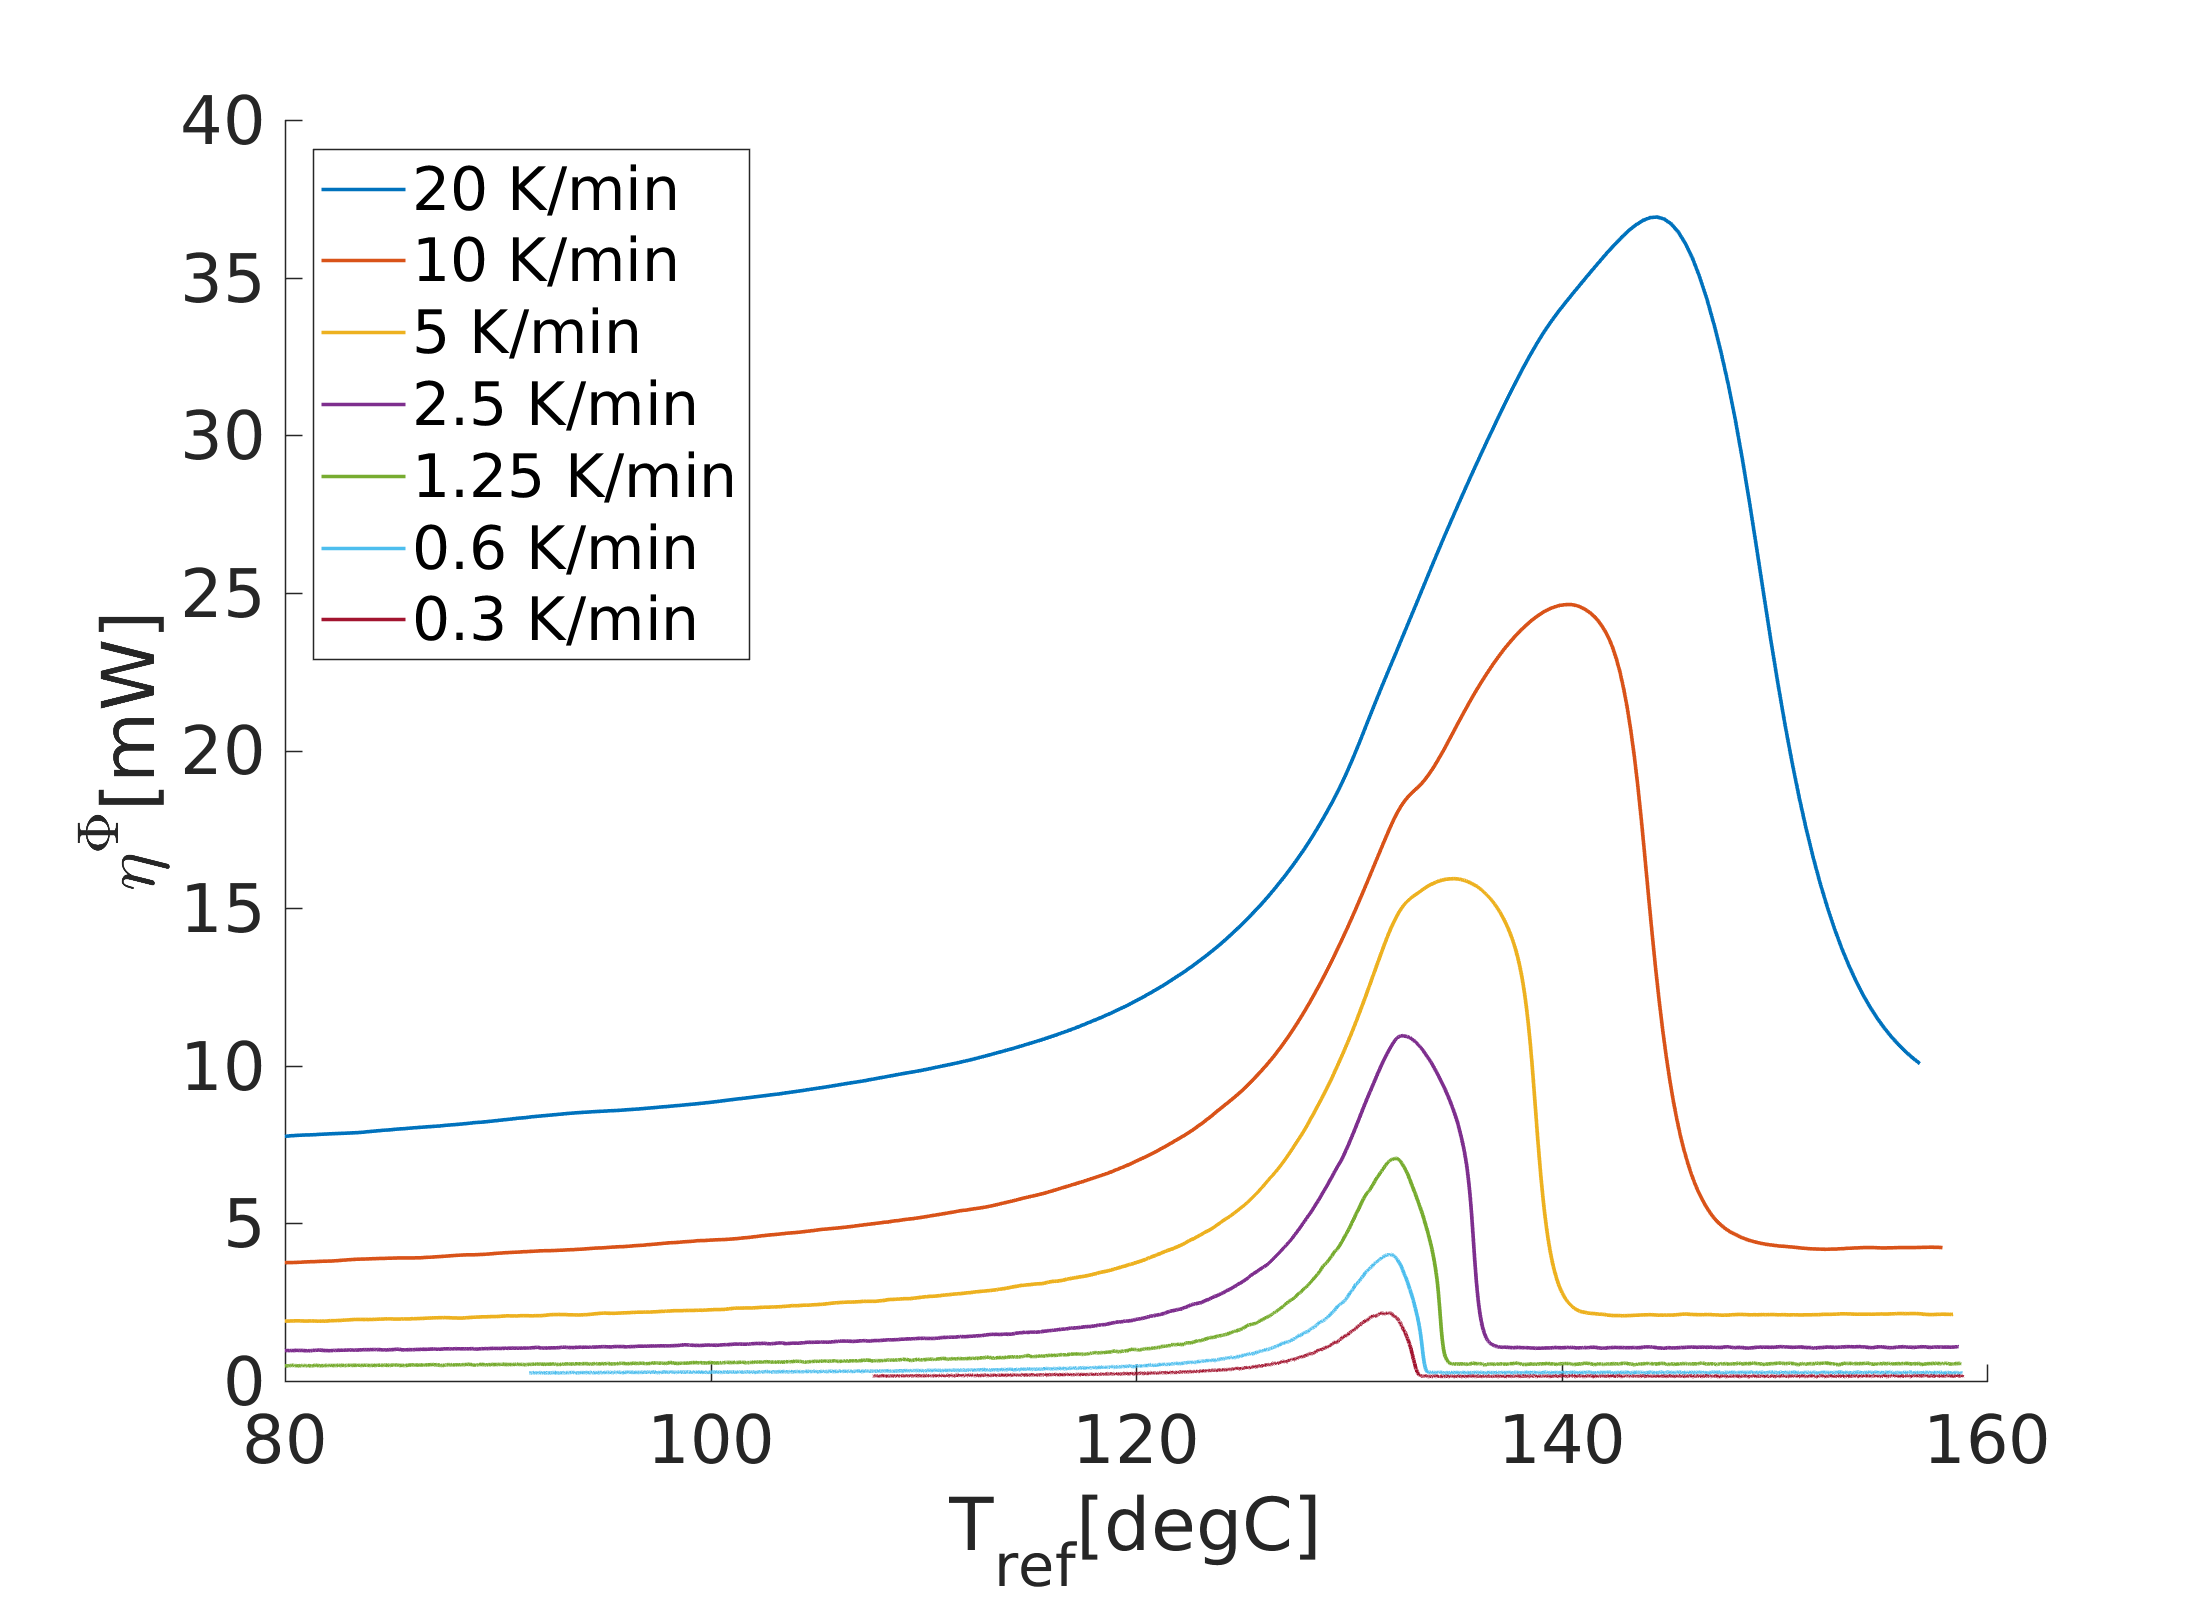
\includegraphics[width=0.7\textwidth]{/home/argo/masterarbeit/vortrag/images/heat_flux_measurement.png}
	\end{textblock}
	
	\begin{textblock}{4}(7.5,8)
		$\stackrel{(1)}{\longrightarrow}$
	\end{textblock}
	
	\begin{textblock}{10}(8.7,5)
		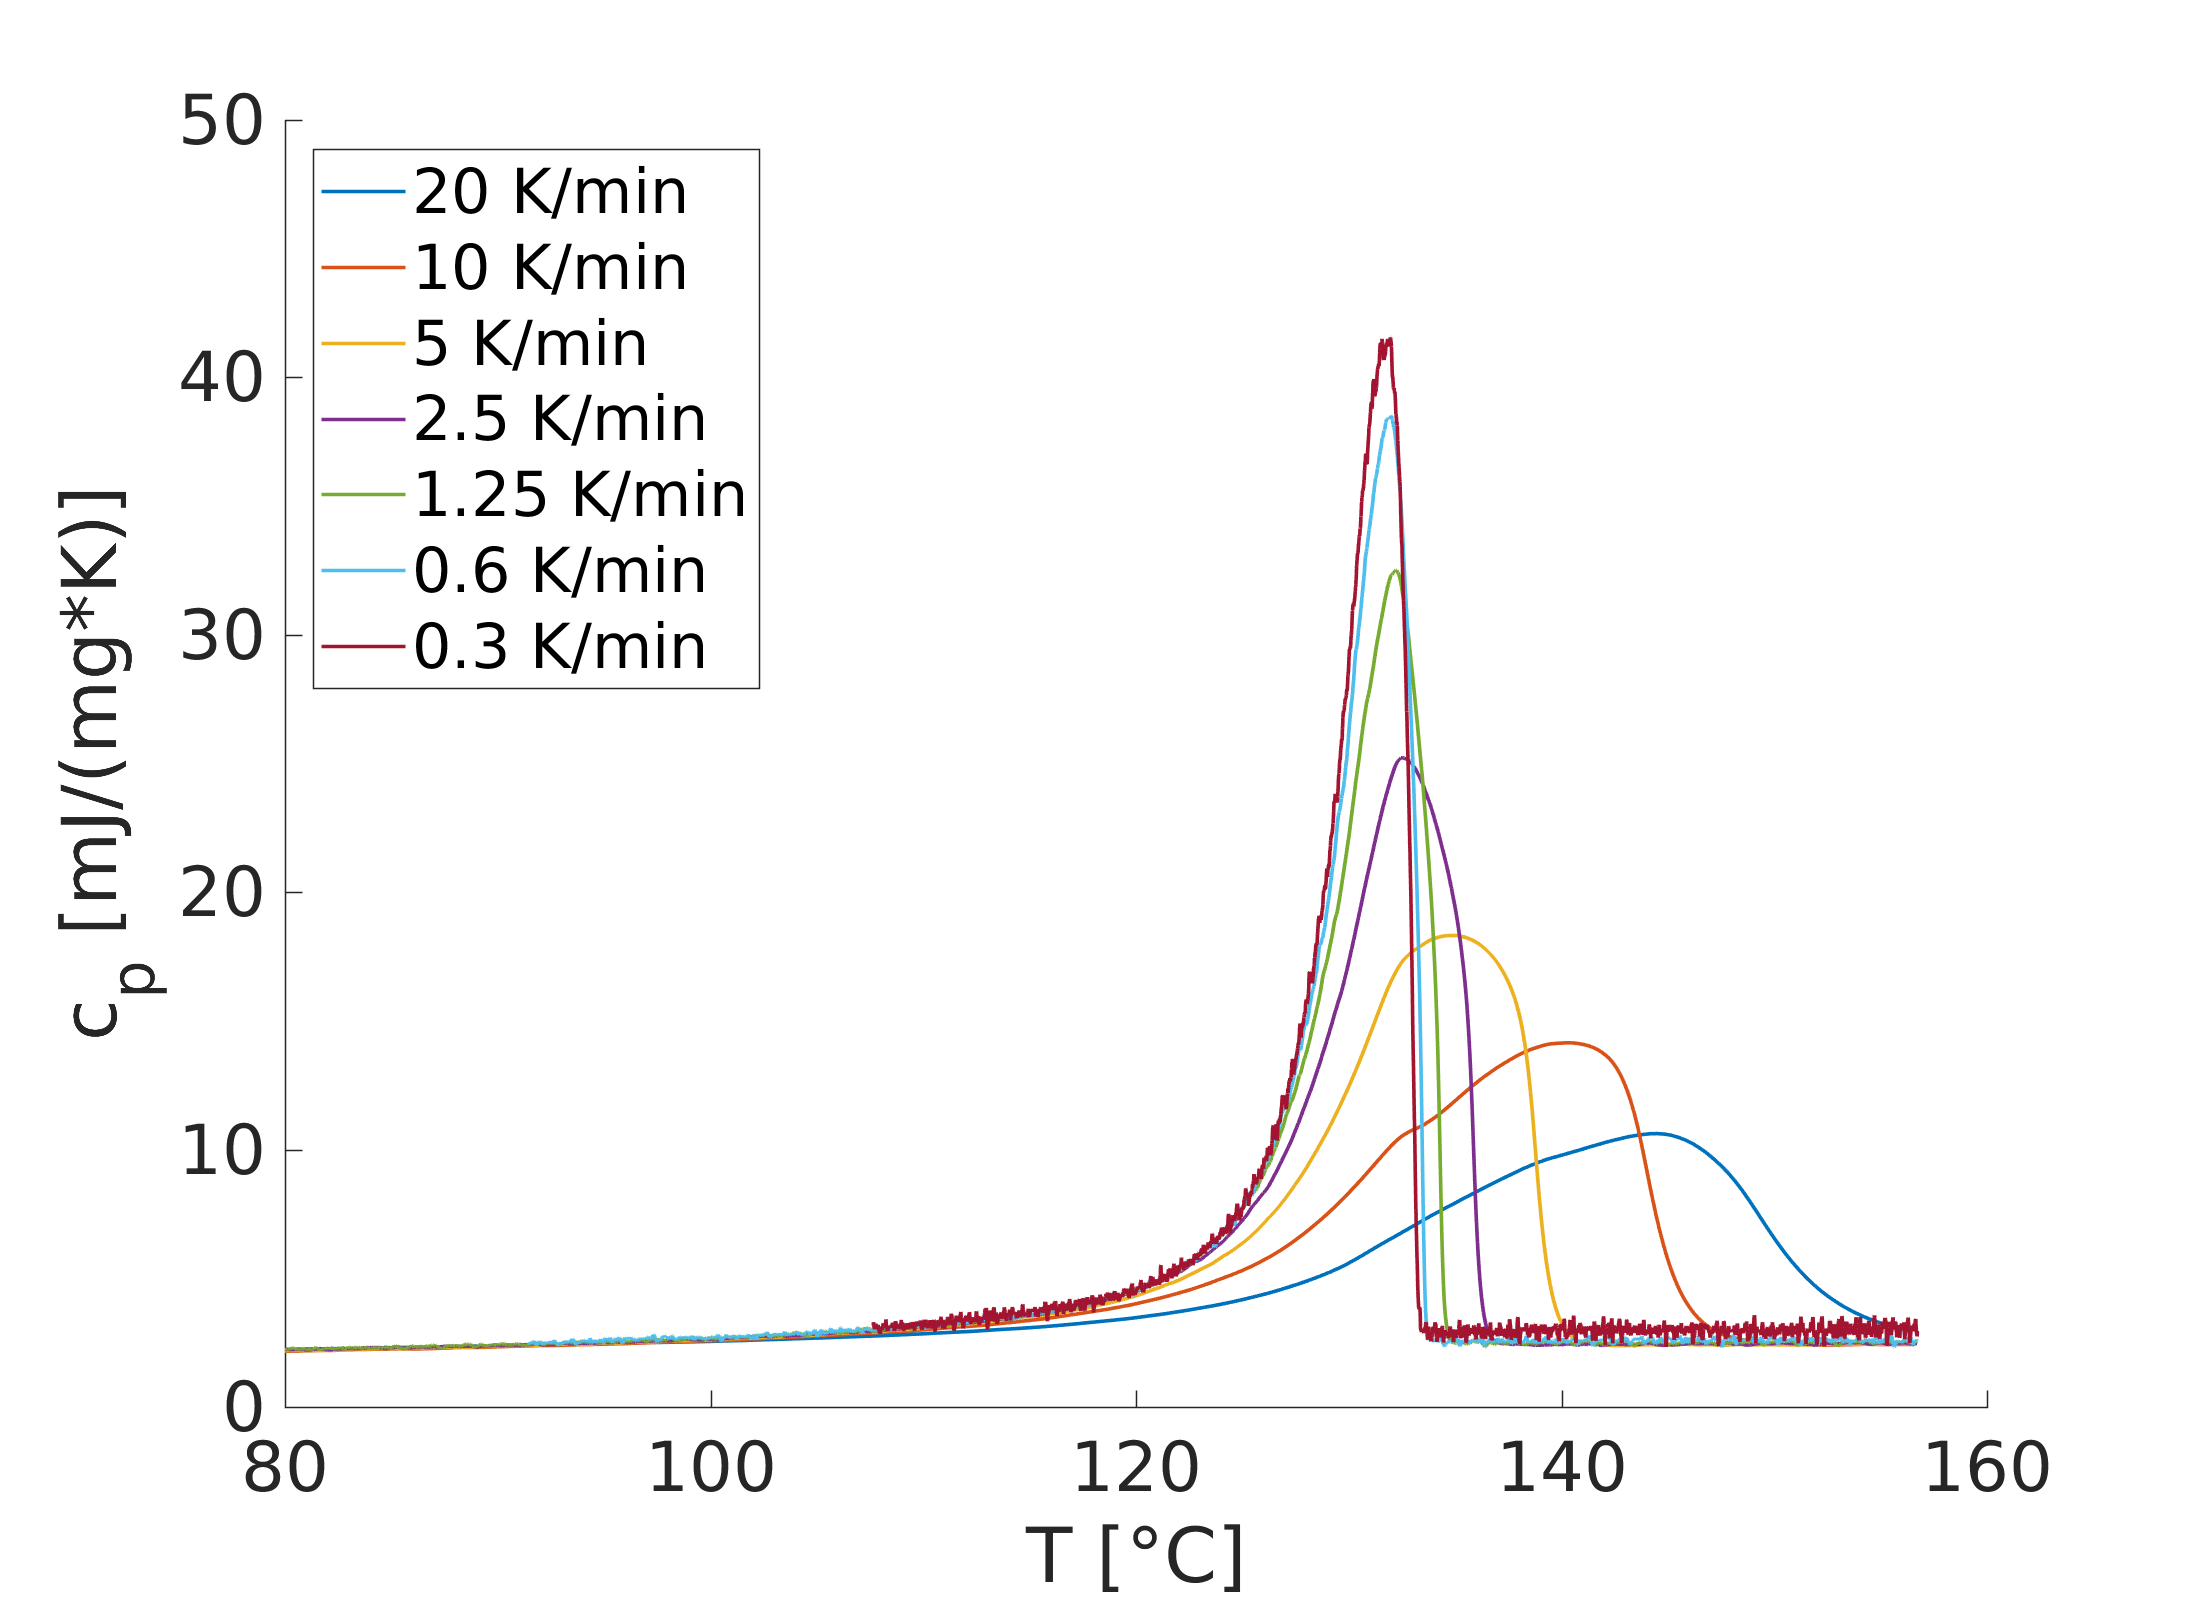
\includegraphics[width=0.7\textwidth]{/home/argo/masterarbeit/vortrag/images/c_p_DIN_formula.png}
	\end{textblock}
	
	\begin{textblock}{14}(1,12)
		\begin{equation}
			\text{DIN 11357: } \quad c_p^{DIN}(T) = c_p^{R}(T) \cdot \frac{m^R}{m^S} \cdot \frac{\Phi^S(T) - \Phi^0(T)}{\Phi^R(T) - \Phi^0(T)}
		\end{equation}
	\end{textblock}
	
}


\section{Mathematical model \& parameter estimation}
\frame{
	\frametitle{Existing similar model --- Dissertation Stefan Hiebler \cite{diss_dsc}}
	
	\begin{textblock}{15}(0.3, 4.5)
		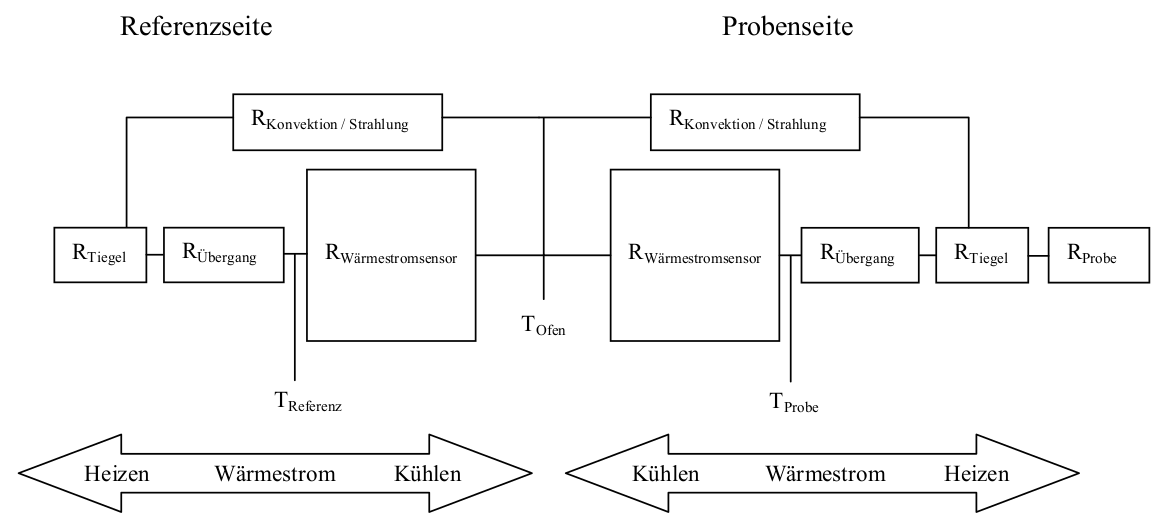
\includegraphics[width=1.\textwidth]{/home/argo/masterarbeit/vortrag/images/diss_dsc_widerstand_schaltbild.png}
	\end{textblock}

	
}

\frame{
	\frametitle{Existing similar model --- Dissertation Stefan Hiebler \cite{diss_dsc}}
	
	\begin{textblock}{13}(1, 5)
		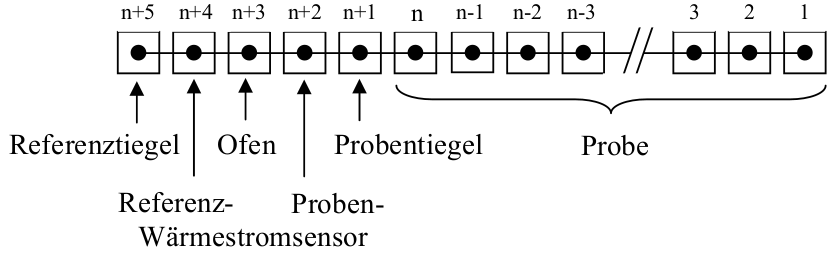
\includegraphics[width=1.\textwidth]{/home/argo/masterarbeit/vortrag/images/diss_dsc_diskretisierung.png}
	\end{textblock}
	
	\begin{textblock}{13}(1,11)
		\begin{itemize}
			\item Heat resistors $R$ are obtained by calibration measurement with Indium \\
			$\rightarrow$ Such measurement data is not available for us
		\end{itemize}
	\end{textblock}
	
}



\subsection{Mathematical model}
\frame{
	\frametitle{Developed mathematical model}
	
	\begin{textblock}{14}(1, 3.9)
		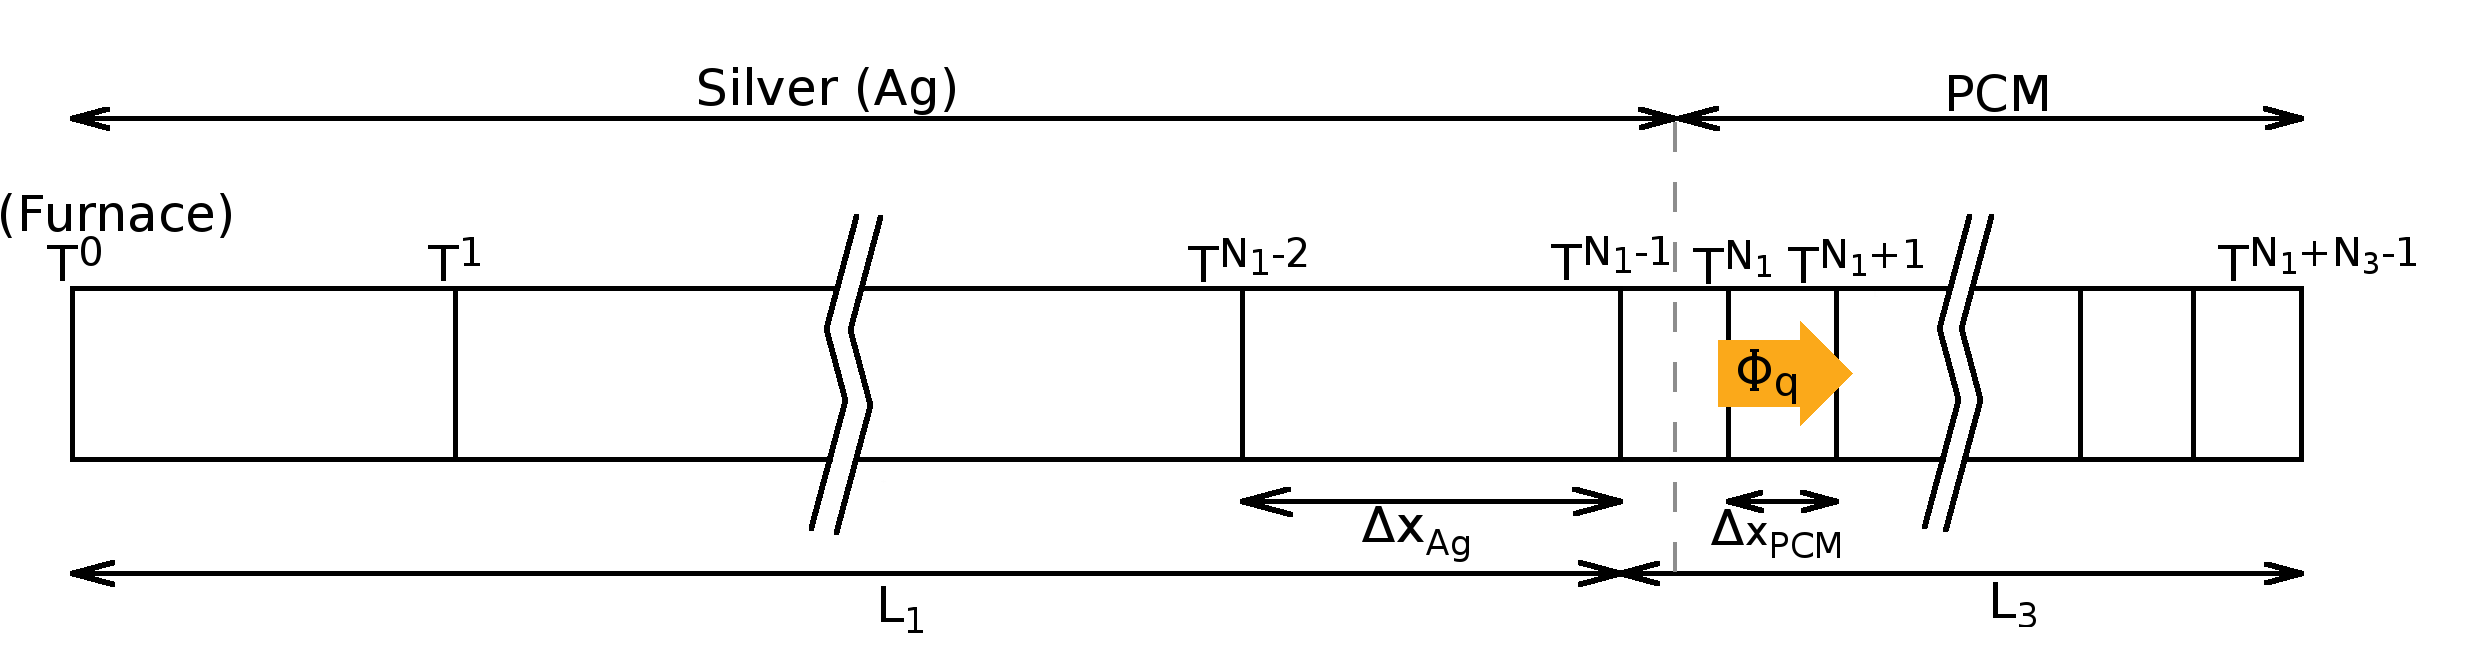
\includegraphics[width=1.\textwidth]{/home/argo/masterarbeit/thesis/images/discretization_grid_heat_flux.png}
	\end{textblock}
	
	
	\begin{textblock}{14}(0.4, 8.8)
	
		\begin{itemize}
			\item Heat equation: \quad $\rho c_p(T(x,t)) \frac{\partial T}{\partial t}(x,t) = \nabla \cdot \left[ \lambda \cdot \nabla T(x,t) \right]$
			\item $\rho$, $\lambda$ constant
			\item Boundary conditions: 
				\begin{itemize}
				\item $T^0 = T_0 + \beta \cdot t$ \\
				\item No flux outside PCM
				\end{itemize}
			\item Reference and PCM side are independent
			\item Spatial discretization by method of lines
			
		\end{itemize}
	\end{textblock}
	
	\begin{textblock}{7}(8,10.35)
		\begin{itemize}
			\item Initial condition: 
			\begin{itemize}
				\item $T^i(t_0)=T_0 \ \forall \ i$
			\end{itemize}
		\end{itemize}
	\end{textblock}

	
}


\frame{

	\begin{textblock}{12}(1.8, 2.5)
		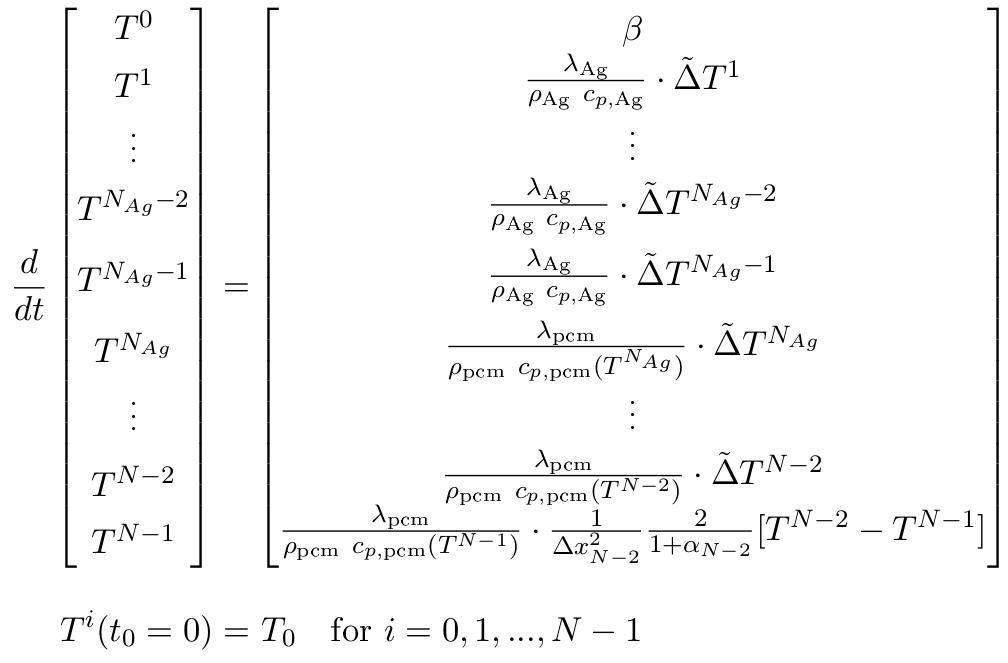
\includegraphics[width=1.0\textwidth]{/home/argo/masterarbeit/vortrag/images/model_IVP.png}
	\end{textblock}
	
	\begin{textblock}{12}(1,13.5)
		 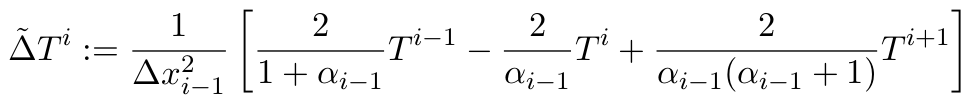
\includegraphics[width=1.0\textwidth]{/home/argo/masterarbeit/vortrag/images/discretized_2nd_derivative_in_IVP.png}
	\end{textblock}
}


\frame{
	\frametitle{Heat flux computation}	
	
	\begin{textblock}{14}(1,4.5)
		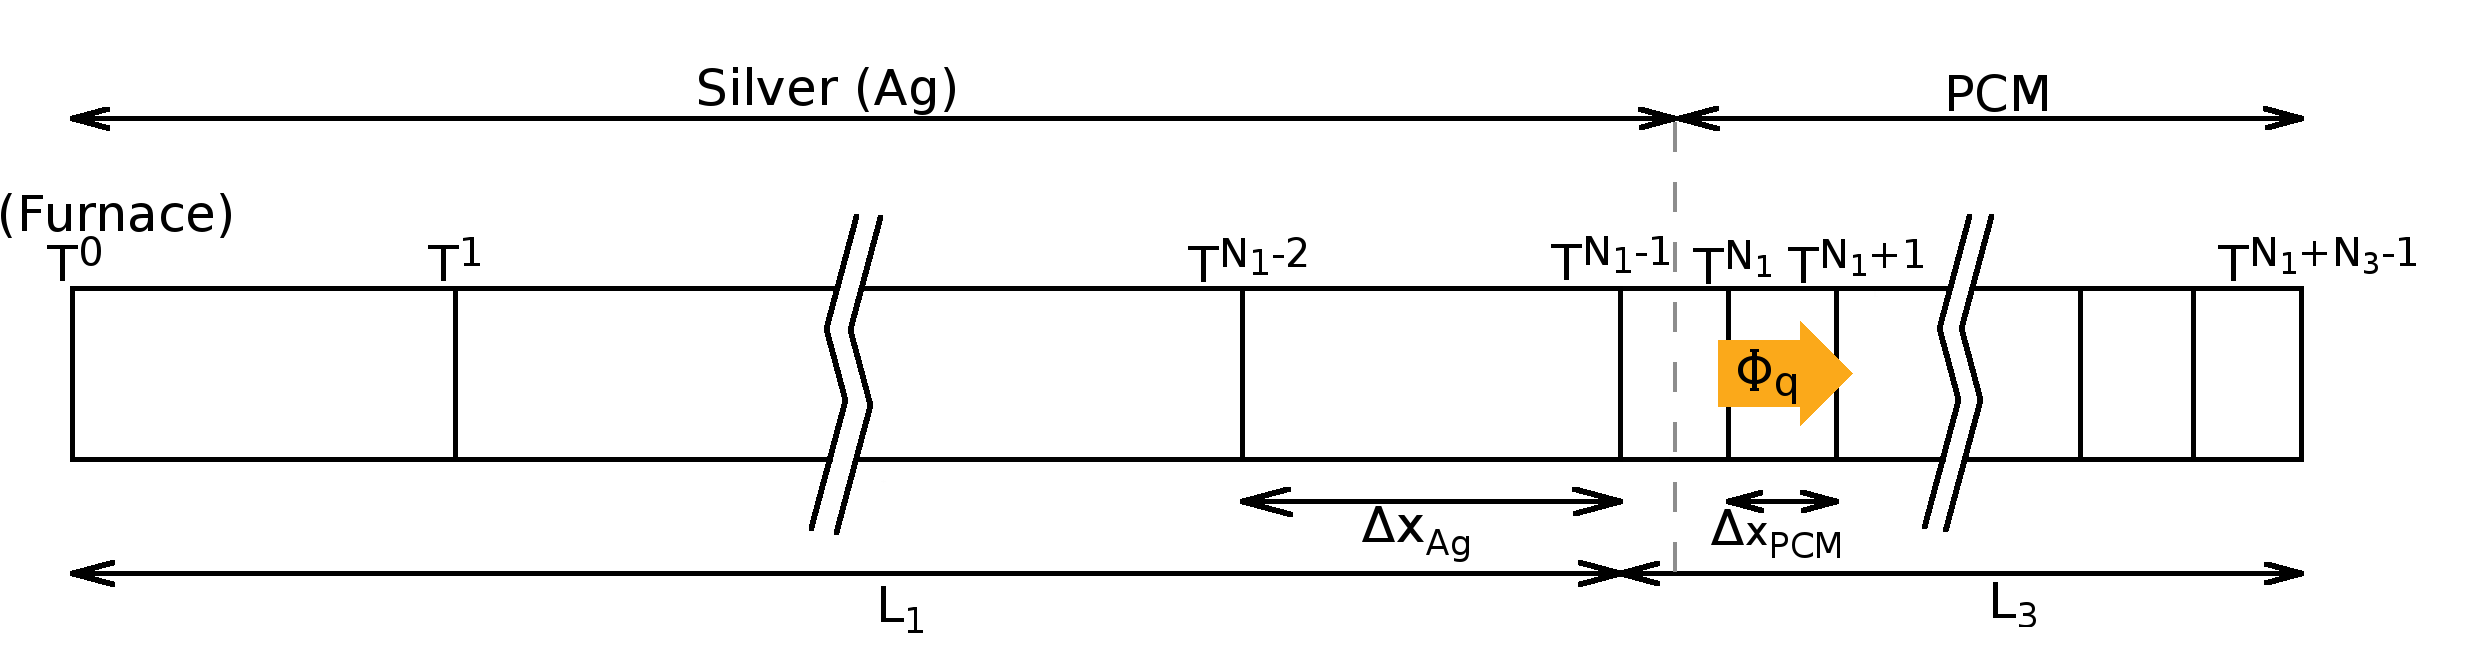
\includegraphics[width=1.\textwidth]{/home/argo/masterarbeit/thesis/images/discretization_grid_heat_flux.png}
	\end{textblock}
	
	\begin{textblock}{14}(1, 10)
		\begin{itemize}
			\item Heat flux into PCM: \\ \vspace{0.15cm}
			$\varPhi_{q}^{pcm,in} \approx - \bar{\lambda} \frac{T^{N_{Ag}} - T^{N_{Ag}-1}}{\Delta x_{N_{Ag}-1}} \cdot A_{pcm}
			\approx - \lambda_{pcm} \frac{T^{N_{Ag}+1} - T^{N_{Ag}}}{\Delta x_{N_{Ag}}} \cdot A_{pcm}$ \\ \vspace{0.15cm}
			where for the cross section $A_{pcm}$ we used $m_{N_{Ag}} = \rho_{pcm} \cdot A_{pcm} \cdot \Delta x_{N_{Ag}}$
		\end{itemize}
	\end{textblock}
	
}



%\frame{
%	\frametitle{Grid generation}
%
%	\begin{textblock}{10}(0.5,5)
%		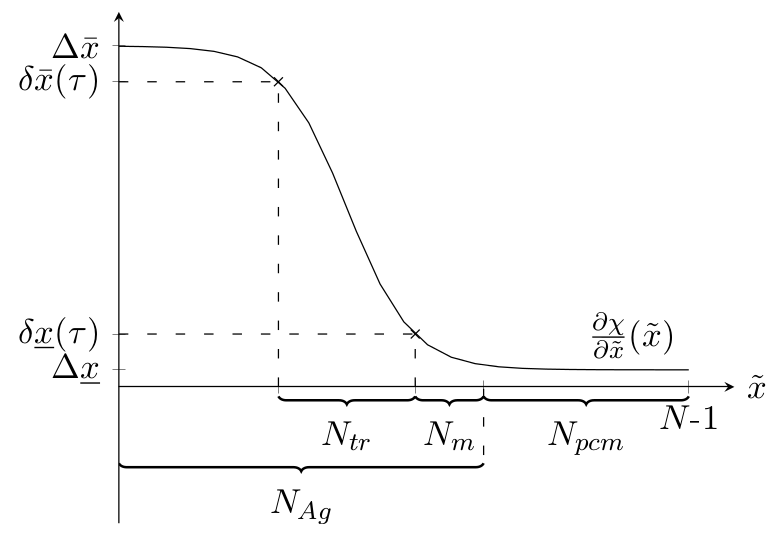
\includegraphics[width=1.0\textwidth]{/home/argo/masterarbeit/vortrag/images/grid_generation.png}
%	\end{textblock}
%	
%}




\subsection{Parametrization $c_p(T)$}
\frame{
	\frametitle{Parametrization $c_p(T)$}	

	\begin{textblock}{14}(1,5)
		\begin{itemize}
			\item Used parametrizations of specific heat capacity function $c_p(T)$ in this thesis:  \\[0.4ex]
			\begin{itemize}
				\item Non-Uniform Rational B-Splines (NURBS) \\[0.7ex]
				\item Linear combination of Gaussians \\[0.7ex]
				\item Fraser-Suzuki Peak 
			\end{itemize}
		\end{itemize}
	\end{textblock}	
		
}





\frame{
	\frametitle{Parametrization $c_p(T)$ --- Linear combination of Gaussians}
	
	\begin{textblock}{14}(1,4.5)
		\begin{equation*}
			c_p(T) = \sum_{i=1}^{5} A_i \exp\left(- \frac{(T - T_{\text{offset}_i})^2}{\var_i}\right) + m \cdot T + b
		\end{equation*}
	\end{textblock}
	
	\begin{textblock}{8}(1,7)
		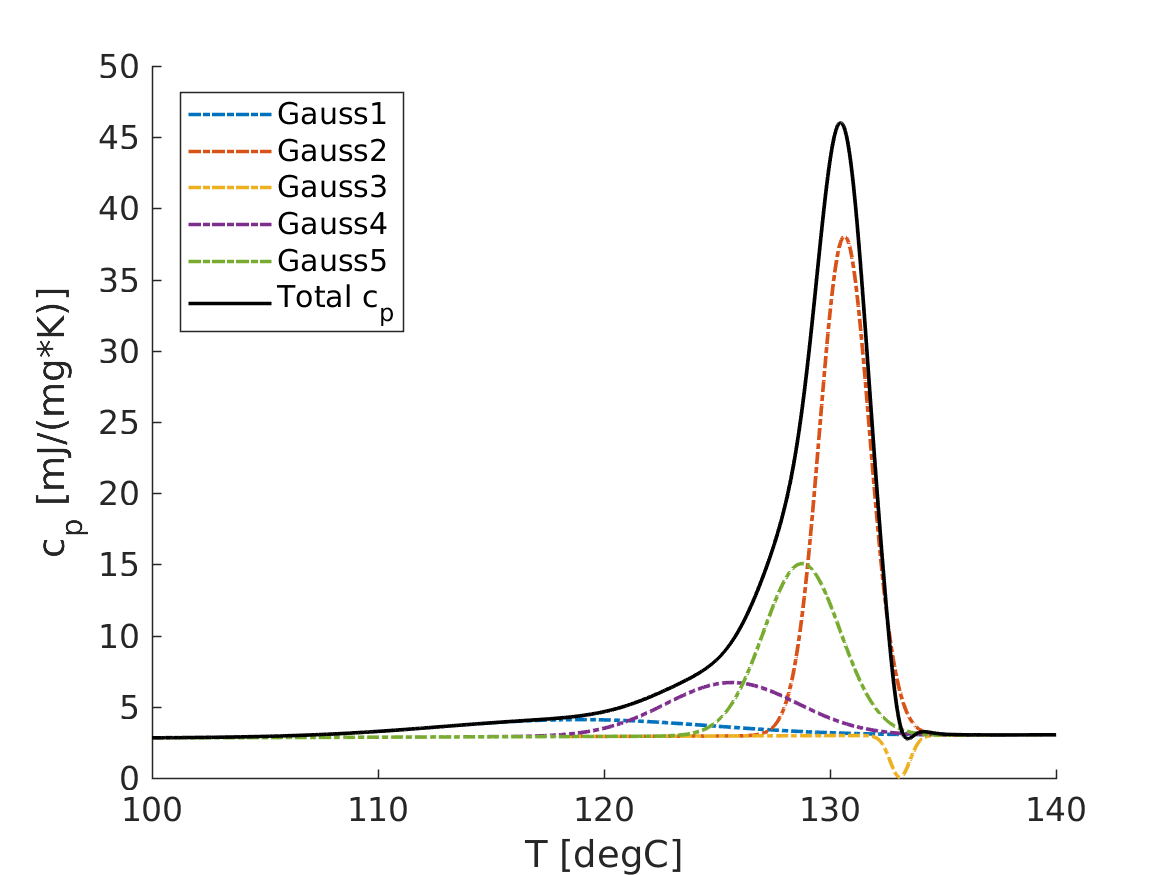
\includegraphics[width=1.0\textwidth]{/home/argo/masterarbeit/thesis/images/c_p_example.png}
	\end{textblock}
	
	\begin{textblock}{7}(8.5,7)
		\begin{itemize}
			\item Parameter: \\
			$A_i$, $T_{offset_i}$ and $\var_i$ for Gaussian i \\
			$m$ and $b$ for linear baseline
			\item In total $17$ parameter 
		\end{itemize}
	\end{textblock}
	
}


\frame{
	\frametitle{Parametrization $c_p(T)$ --- Fraser-Suzuki peak}
	
	\begin{textblock}{15.5}(0.2,4.3)
		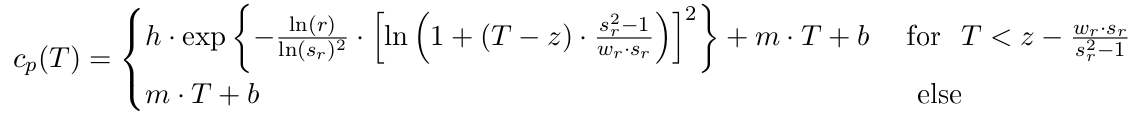
\includegraphics[width=1.0\textwidth]{/home/argo/masterarbeit/vortrag/images/fs_formula.png}
	\end{textblock}
	
	\begin{textblock}{8}(0.5,7)
		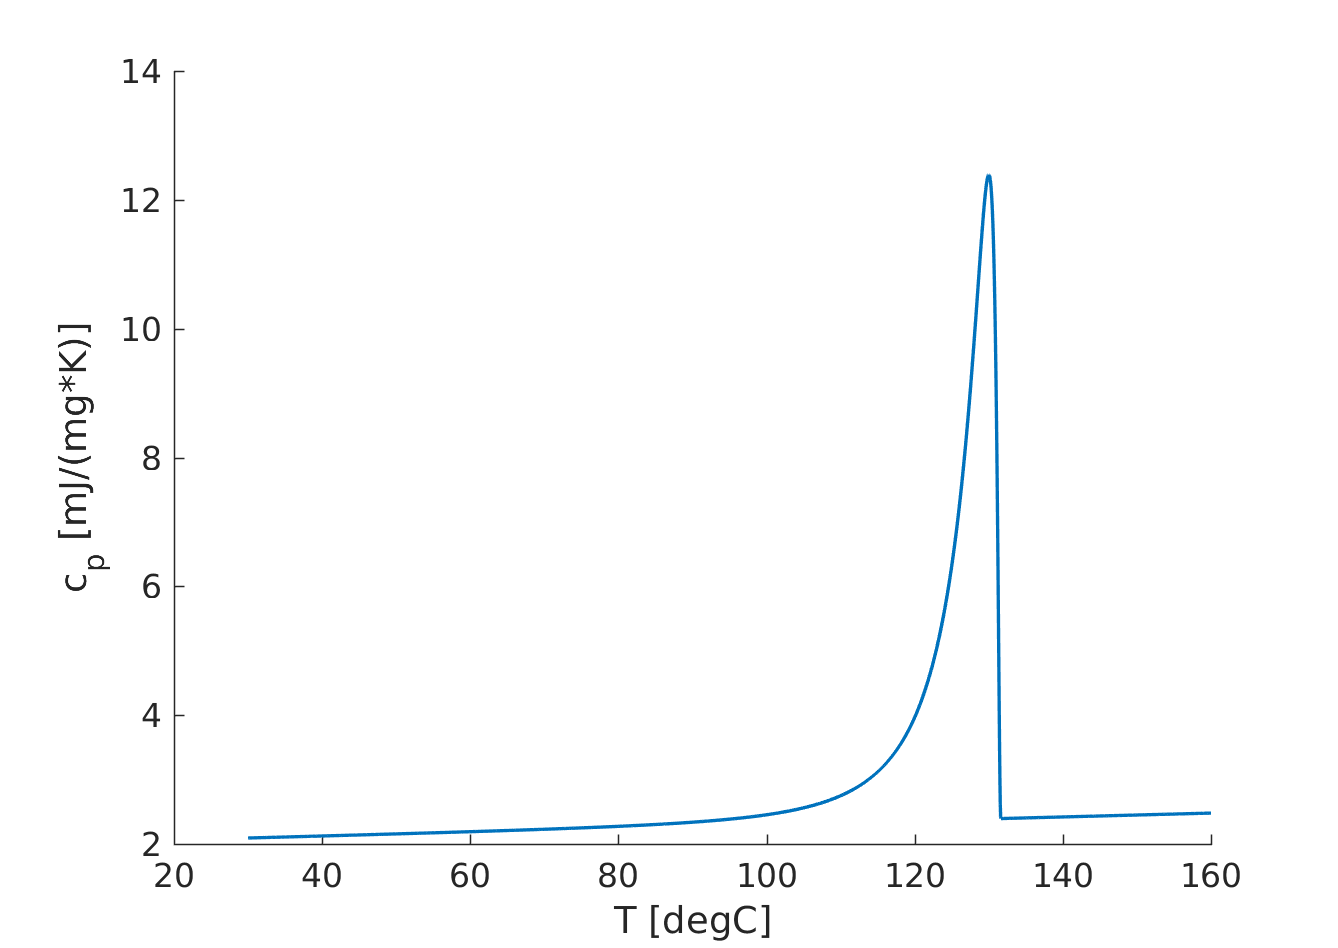
\includegraphics[width=1.0\textwidth]{/home/argo/masterarbeit/thesis/images/fraser_suzuki_example.png}
	\end{textblock}
	
	\begin{textblock}{7}(8.5,8)
		\begin{itemize}
			\item Parameter: \\
			$h$, $w_r$, $s_r$, $z$ for \\
			Fraser-Suzuki peak
			\item fixed $r=2$ for identifiability
			\item $m$ and $b$ for linear baseline
			\item In total $6$ parameter 
		\end{itemize}
	\end{textblock}
	
}




\subsection{Optimization problem}


\frame{
	\frametitle{Computation of measurement time points}
	
	\begin{textblock}{8.5}(0.35,5)
		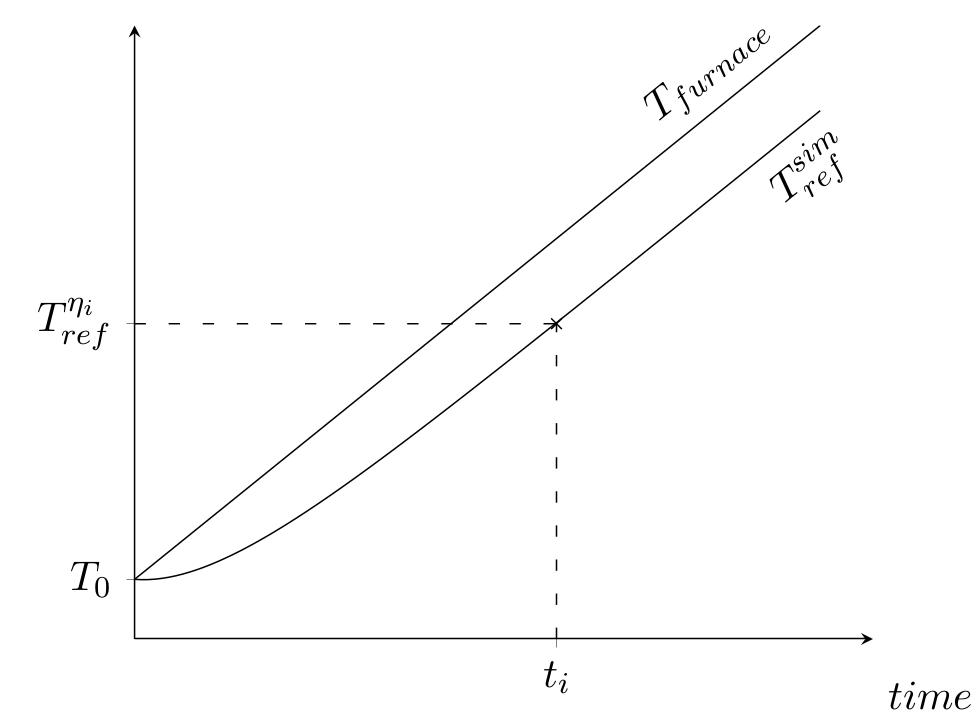
\includegraphics[width=1.\textwidth]{/home/argo/masterarbeit/vortrag/images/measurement_time_computation2.png}
	\end{textblock}
	
	\begin{textblock}{6.8}(8.5,5.)
	\begin{itemize}
		\item Reference side $T_{ref}^{sim}(t)$ is solved analytically \\[2ex]
		\item Given heat flux measurement values $\varPhi_q^{\eta_i} = \varPhi_q^{\eta_i}(T_{ref}^{\eta_i})$ \\[1ex]
		$\rightarrow$ For fixed $T_0$ we can compute points in time $t_i$ where measurements were done using Newton's method
	\end{itemize}
	\end{textblock}

	
}



\frame{
	\frametitle{Optimization problem}	


	\begin{textblock}{10}(0.5,3.5)
	\begin{align*}
		\min_{p_{c_p}} \ & \sum_{i=1}^{n_{mp}} \left(  \varPhi_{q}^{pcm,in}(T(t_i;T_0,p_{c_p})) - \varPhi_q^{\eta_i} \right)^2 \\
		s.t. \ & \quad \  \dot{T} = f(T,t;p_{c_p}) \\
		       & T(0) = T_0 \\
		       & \underline{p} \le p_{c_p} \le \bar{p}
	\end{align*}
	\end{textblock}
	
	\begin{textblock}{7}(12,6.7)
		separately for all \\
		 heat rates $\beta$
	\end{textblock}
	
	\begin{textblock}{16}(0.3,9.4)
	\begin{itemize}
		\item $\varPhi_q^{\eta_i}$: heat flux measurement value at time $t_i$
		\item $\varPhi_q^{\text{pcm,in}}$: heat flux into PCM from simulation \\
		\item $n_{mp}$: number of measurement points \\
		\item $p_{c_p}$: optimization parameters specifying specific heat capacity $c_p(T)$ \\
		\item $f(T,t;p_{c_p})$: discretized differential equation system from heat equation
	\end{itemize}
	
	\end{textblock}

	
}





\section{Numerical experiments and results}

\subsection{Gaussian parametrization}
\frame{
	\frametitle{Numerical experiments --- Gaussian parametrization}
	
	\begin{textblock}{14}(1,5)
		\begin{itemize}
			\item Software: SolvIND using integrator DAESOL-II \\ \vspace{0.15cm}
			$\rightarrow$ Computes as well needed sensitivities $\frac{\partial T}{\partial p}$ for optimization \\
			\qquad using AD in forward mode
			\item Used relative local integration tolerance: $10^{-7}$
			\item Nonlinear least squares solver: Matlab routine $lsqnonlin$
		\end{itemize}
	\end{textblock}	
}


\frame{
	\frametitle{Linear combination of Gaussians}
	
	\begin{textblock}{14}(1,4.5)
		\begin{equation*}
		c_p(T) = \sum_{i=1}^{5} A_i \exp\left(- \frac{(T - T_{\text{offset}_i})^2}{\var_i}\right) + m \cdot T + b
		\end{equation*}
	\end{textblock}
	
	\begin{textblock}{8}(1,7)
		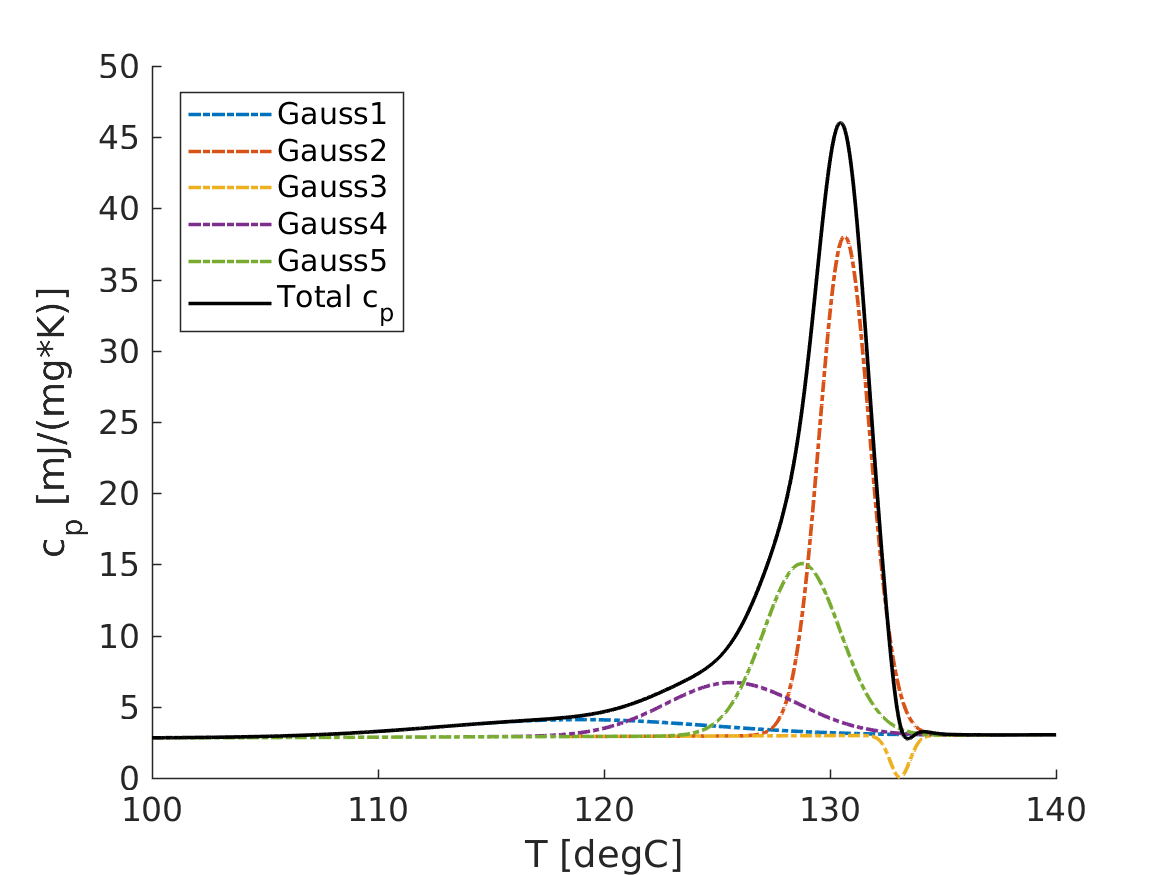
\includegraphics[width=1.0\textwidth]{/home/argo/masterarbeit/thesis/images/c_p_example.png}
	\end{textblock}
	
	\begin{textblock}{7}(8.5,7)
		\begin{itemize}
			\item Parameter: \\
			$A_i$, $T_{offset_i}$ and $\var_i$ for Gaussian i \\
			$m$ and $b$ for linear baseline
			\item In total $17$ parameter 
		\end{itemize}
	\end{textblock}
	
}

\frame{
	\frametitle{Specific heat capacity \& heat flux}
	\begin{textblock}{14}(1,5)
		\centering
		Heat rate: $10\frac{K}{min}$
	\end{textblock}
	
	\begin{textblock}{8}(0.3,6.5)
		\includegraphics[width=1.\textwidth]{/home/argo/masterarbeit/fits_data/2017-12-19_20:27:59_407_L1=40_L3=0.1_N1=300_N3=50_5Gaussians_used/2017-12-19_21:17:51_407_10Kmin_L1=40_L3=0,1/c_p_vortrag2.png}
	\end{textblock}
	
	\begin{textblock}{8}(8.2,6.7)
		\includegraphics[width=1.\textwidth]{/home/argo/masterarbeit/fits_data/2017-12-19_20:27:59_407_L1=40_L3=0.1_N1=300_N3=50_5Gaussians_used/2017-12-19_21:17:51_407_10Kmin_L1=40_L3=0,1/heat_flux_vortrag2.png}
	\end{textblock}	
}


\frame{
	\frametitle{Specific heat capacity \& heat flux}
	\begin{textblock}{15}(0.5,5)
		\centering
		Heat rate: $5\frac{K}{min}$
	\end{textblock}
	
	\begin{textblock}{8}(0.3,6.5)
		\includegraphics[width=1.\textwidth]{/home/argo/masterarbeit/fits_data/2017-12-19_20:27:59_407_L1=40_L3=0.1_N1=300_N3=50_5Gaussians_used/2017-12-19_21:44:04_407_5Kmin_L1=40_L3=0,1/c_p_vortrag2.png}
	\end{textblock}
	
	\begin{textblock}{8}(8.2,6.7)
		\includegraphics[width=1.\textwidth]{/home/argo/masterarbeit/fits_data/2017-12-19_20:27:59_407_L1=40_L3=0.1_N1=300_N3=50_5Gaussians_used/2017-12-19_21:44:04_407_5Kmin_L1=40_L3=0,1/heat_flux_vortrag2.png}
	\end{textblock}	
}


\frame{
	\frametitle{Statistical a posteriori analysis \& [NOC1]}	
	
	\begin{textblock}{14}(1.,4.5)
		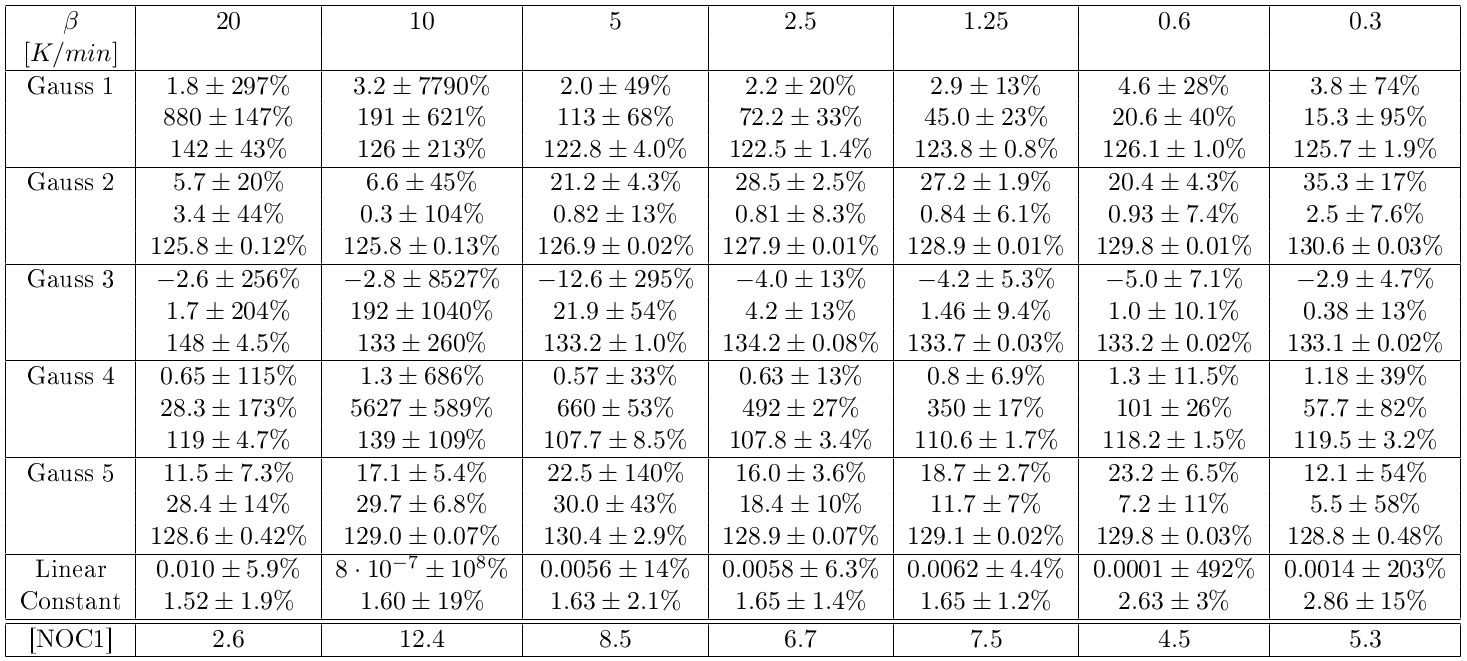
\includegraphics[width=1.\textwidth]{/home/argo/masterarbeit/vortrag/images/stat_a_post_analysis_Gausse.png}
	\end{textblock}	
	
	\begin{textblock}{14}(1.,13.5)
		\begin{itemize}
%			\item $G_L(\alpha) \subset [p_1-\theta_1,p_1+\theta_1] \times ... \times [p_{n_p}-\theta_{n_p},p_{n_p}+\theta_{n_p}]$
			\item Probability of error: $5\%$
		\end{itemize}
	\end{textblock}
	
%	\begin{textblock}{8}(6, 13.)
%		\begin{itemize}
%			\item $G_L(\alpha) \subset [p_1-\theta_1,p_1+\theta_1] \times ... \times [p_{n_p}-\theta_{n_p},p_{n_p}+\theta_{n_p}]$
%		\end{itemize}
%	\end{textblock}
	
}


\subsection{Fraser-Suzuki parametrization}
\frame{
	\frametitle{Numerical experiments --- Fraser-Suzuki parametrization}
	
	\begin{textblock}{14}(1,5)
		\begin{itemize}
			\item Software: SolvIND using integrator DAESOL-II \\ \vspace{0.15cm}
			$\rightarrow$ Computes as well needed sensitivities $\frac{\partial T}{\partial p}$ for optimization \\
			\qquad using AD in forward mode
			\item Relative local integration tolerance: $10^{-9}$
			\item Relative local forward sensitivities tolerance: $5 \cdot 10^{-6}$
			\item Nonlinear least squares solver: Self written Gauss-Newton with linesearch and active set strategy
		\end{itemize}
	\end{textblock}	
}




\frame{
	\frametitle{Fraser-Suzuki peak}
	
	\begin{textblock}{15.5}(0.2,4.3)
		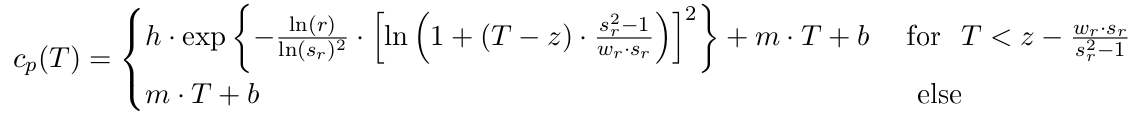
\includegraphics[width=1.0\textwidth]{/home/argo/masterarbeit/vortrag/images/fs_formula.png}
	\end{textblock}
	
	\begin{textblock}{8}(0.5,7)
		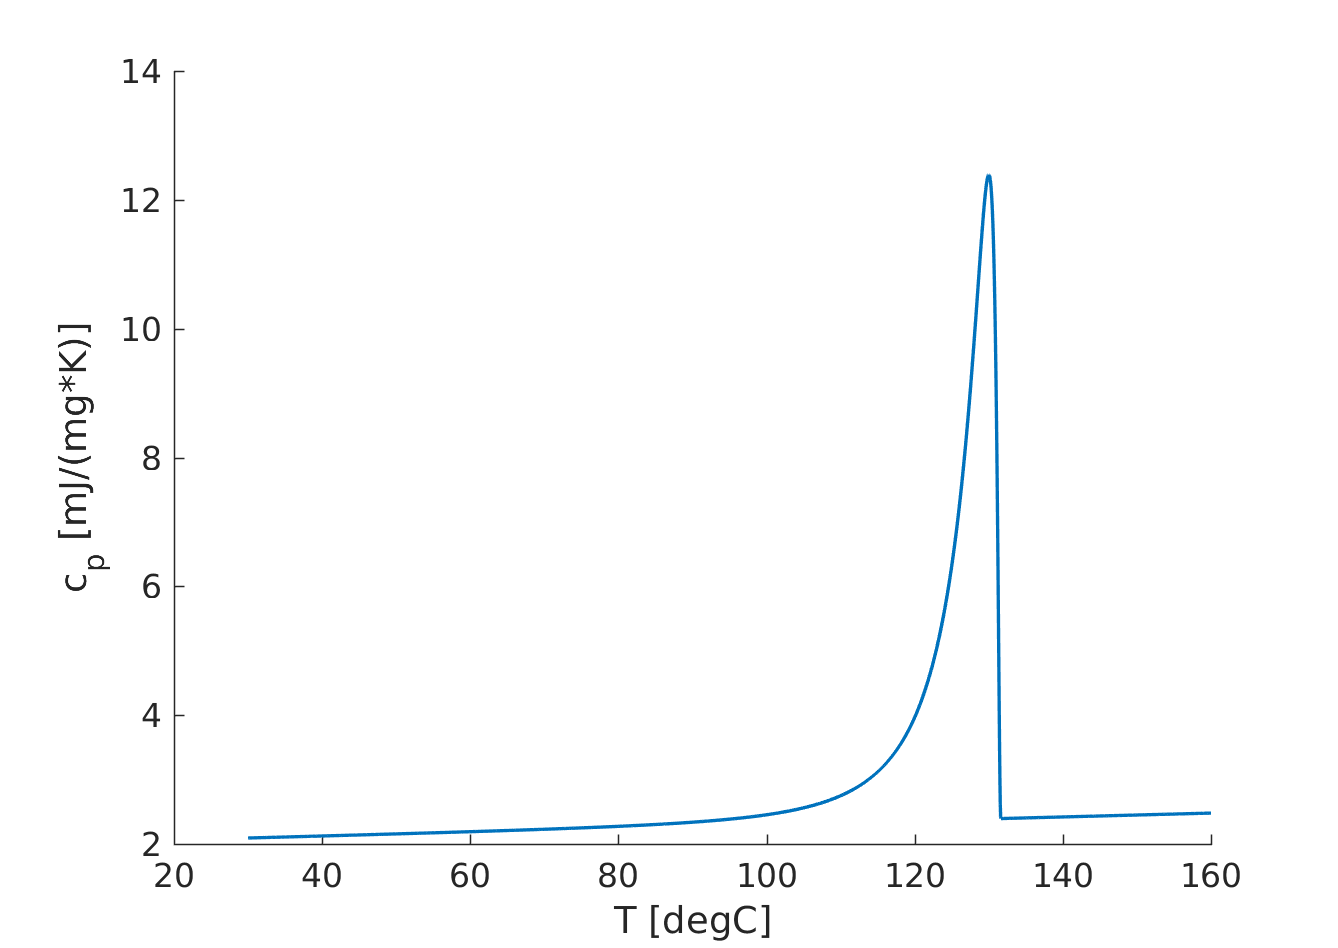
\includegraphics[width=1.0\textwidth]{/home/argo/masterarbeit/thesis/images/fraser_suzuki_example.png}
	\end{textblock}
	
	\begin{textblock}{7}(8.5,8)
		\begin{itemize}
			\item Parameter: \\
			$h$, $w_r$, $s_r$, $z$ for \\
			Fraser-Suzuki peak
			\item fixed $r=2$ for identifiability
			$m$ and $b$ for linear baseline
			\item In total $6$ parameter 
		\end{itemize}
	\end{textblock}
	
}



\frame{
	\frametitle{Specific heat capacity \& heat flux}	
	\begin{textblock}{14}(1,5)
		\centering
		Heat rate: $10\frac{K}{min}$
	\end{textblock}
	
	\begin{textblock}{8}(0.3,6.5)
		\includegraphics[width=1.\textwidth]{/home/argo/masterarbeit/fits_data/2017-12-20_14:25:10_407_L1=40_L3=0,1_N1=300_N3=50_GN_FS_used/2017-12-20_14:30:23_407_10Kmin_L1=40_L3=0,1/c_p_vortrag2.png}
	\end{textblock}
	
	\begin{textblock}{8}(8.2,6.65)
		\includegraphics[width=1.\textwidth]{/home/argo/masterarbeit/fits_data/2017-12-20_14:25:10_407_L1=40_L3=0,1_N1=300_N3=50_GN_FS_used/2017-12-20_14:30:23_407_10Kmin_L1=40_L3=0,1/heat_flux_vortrag2.png}
	\end{textblock}	
	
}


\frame{
	\frametitle{Specific heat capacity \& heat flux}	
	\begin{textblock}{14}(1,5)
		\centering
		Heat rate: $5\frac{K}{min}$
	\end{textblock}
	
	\begin{textblock}{8}(0.3,6.5)
		\includegraphics[width=1.\textwidth]{/home/argo/masterarbeit/fits_data/2017-12-20_14:25:10_407_L1=40_L3=0,1_N1=300_N3=50_GN_FS_used/2017-12-20_14:36:33_407_5Kmin_L1=40_L3=0,1/c_p_vortrag2.png}
	\end{textblock}
	
	\begin{textblock}{8}(8,6.65)
		\includegraphics[width=1.\textwidth]{/home/argo/masterarbeit/fits_data/2017-12-20_14:25:10_407_L1=40_L3=0,1_N1=300_N3=50_GN_FS_used/2017-12-20_14:36:33_407_5Kmin_L1=40_L3=0,1/heat_flux_vortrag2.png}
	\end{textblock}	
	
}

\frame{
	\frametitle{Statistical a posteriori analysis}	
	
	\begin{textblock}{14}(1.,5.)
		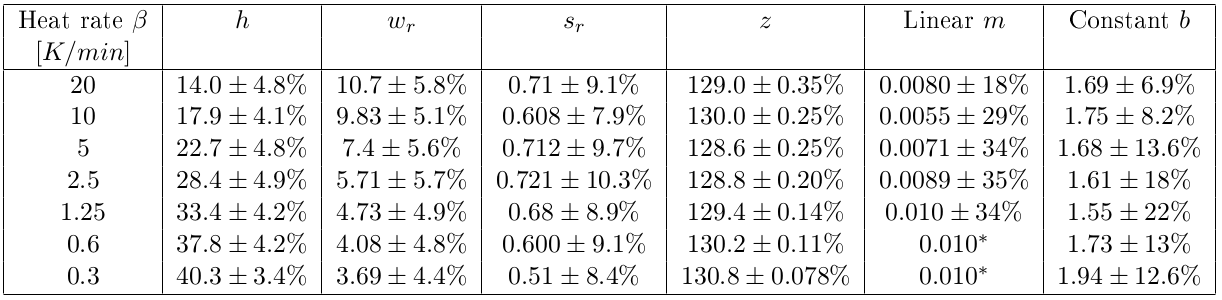
\includegraphics[width=1.\textwidth]{/home/argo/masterarbeit/vortrag/images/stat_a_post_analysis_FS.png}
	\end{textblock}	
	
	\begin{textblock}{15}(0.5,10)
		\begin{itemize}
			\item Probability of error: $5\%$
			\item $^*$ parameter fixed due to lack of measurement data in sensitive part
		\end{itemize}
	\end{textblock}
	
}


\frame{
	\frametitle{Examination of Gauss-Newton iterations}	
	
	\begin{textblock}{8}(0.3,4.5)
		\includegraphics[width=1.\textwidth]{/home/argo/masterarbeit/fits_data/2017-12-20_14:25:10_407_L1=40_L3=0,1_N1=300_N3=50_GN_FS_used/2017-12-20_14:36:33_407_5Kmin_L1=40_L3=0,1/optimization_progress_vortrag.png}
	\end{textblock}
	
	\begin{textblock}{8}(8.2,4.5)
		\includegraphics[width=1.\textwidth]{/home/argo/masterarbeit/fits_data/2017-12-20_14:25:10_407_L1=40_L3=0,1_N1=300_N3=50_GN_FS_used/2017-12-20_14:44:53_407_0,6Kmin_L1=40_L3=0,1/optimization_progress_vortrag.png}
	\end{textblock}
	
}




\subsection{Comparison of retrieved specific heat capacity}

\frame{
	
	\begin{textblock}{6}(0.5, 2.8)
		\underline{Comparison of differently} \\ \underline{computed specific heat}\\ 
		\underline{capacity $c_p(T)$}
	\end{textblock}
	
	\begin{textblock}{6.9}(0,6.5)
		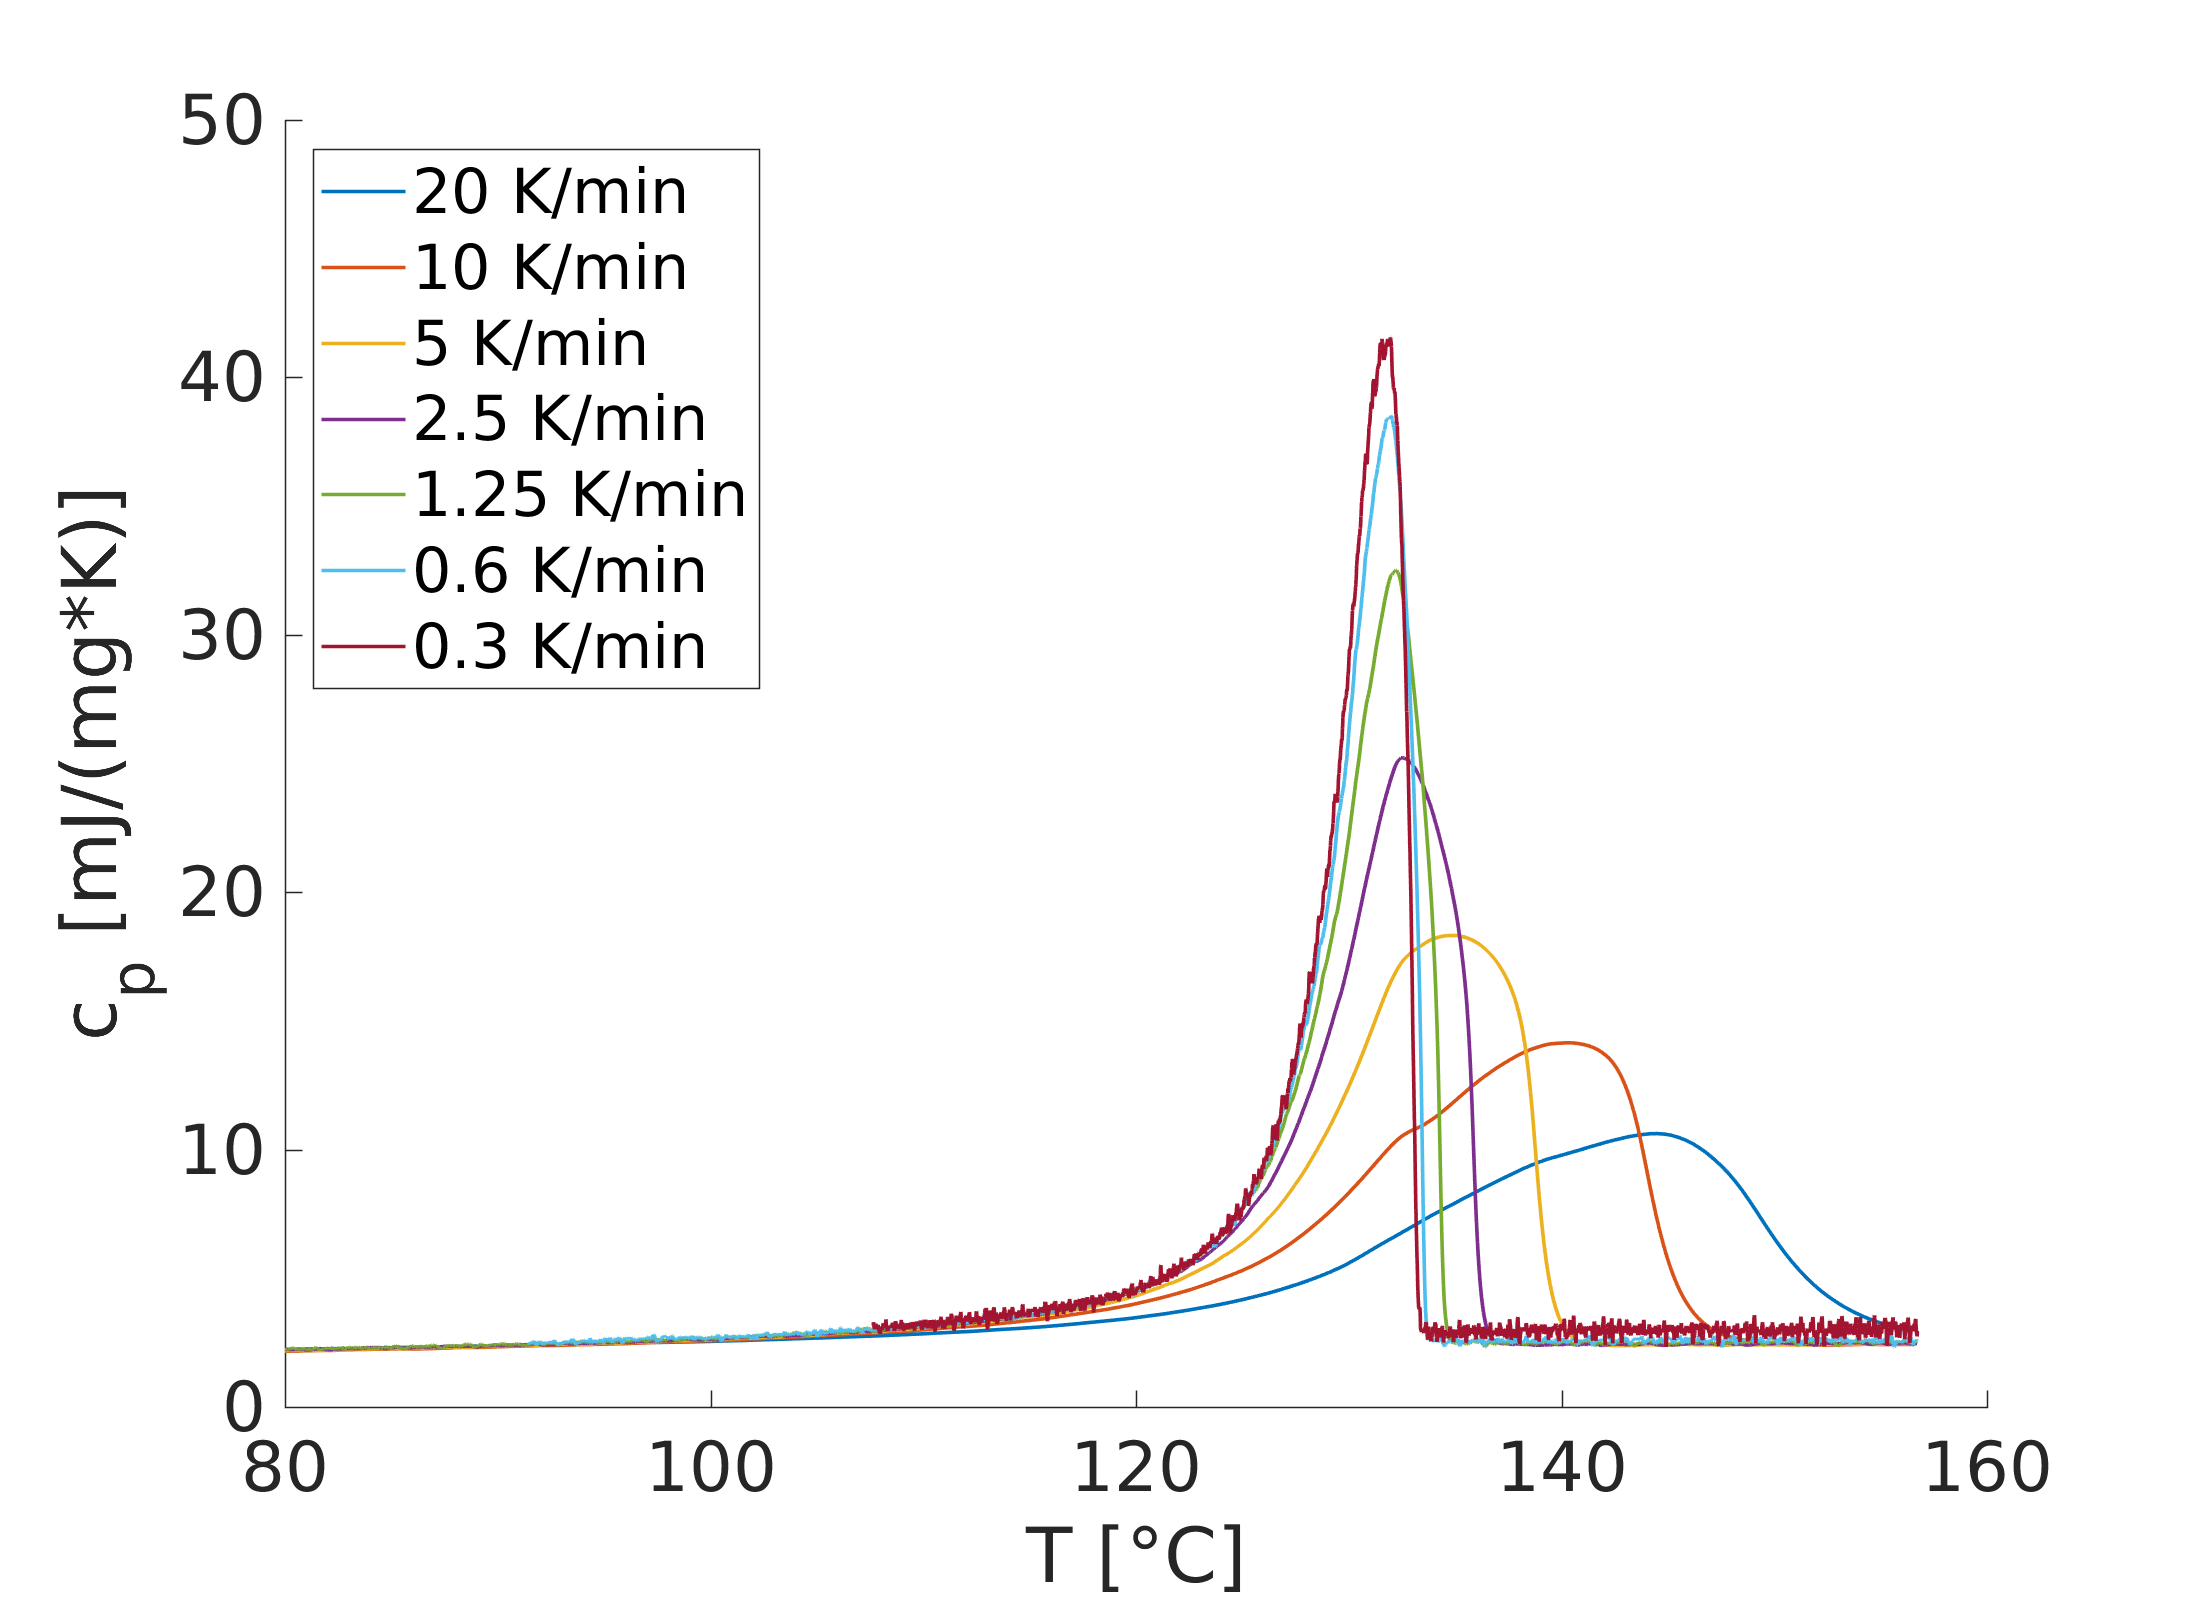
\includegraphics[width=1.\textwidth]{/home/argo/masterarbeit/vortrag/images/c_p_DIN_formula.png}
	\end{textblock}
	
	
	\begin{textblock}{6.9}(8.,2.3)
		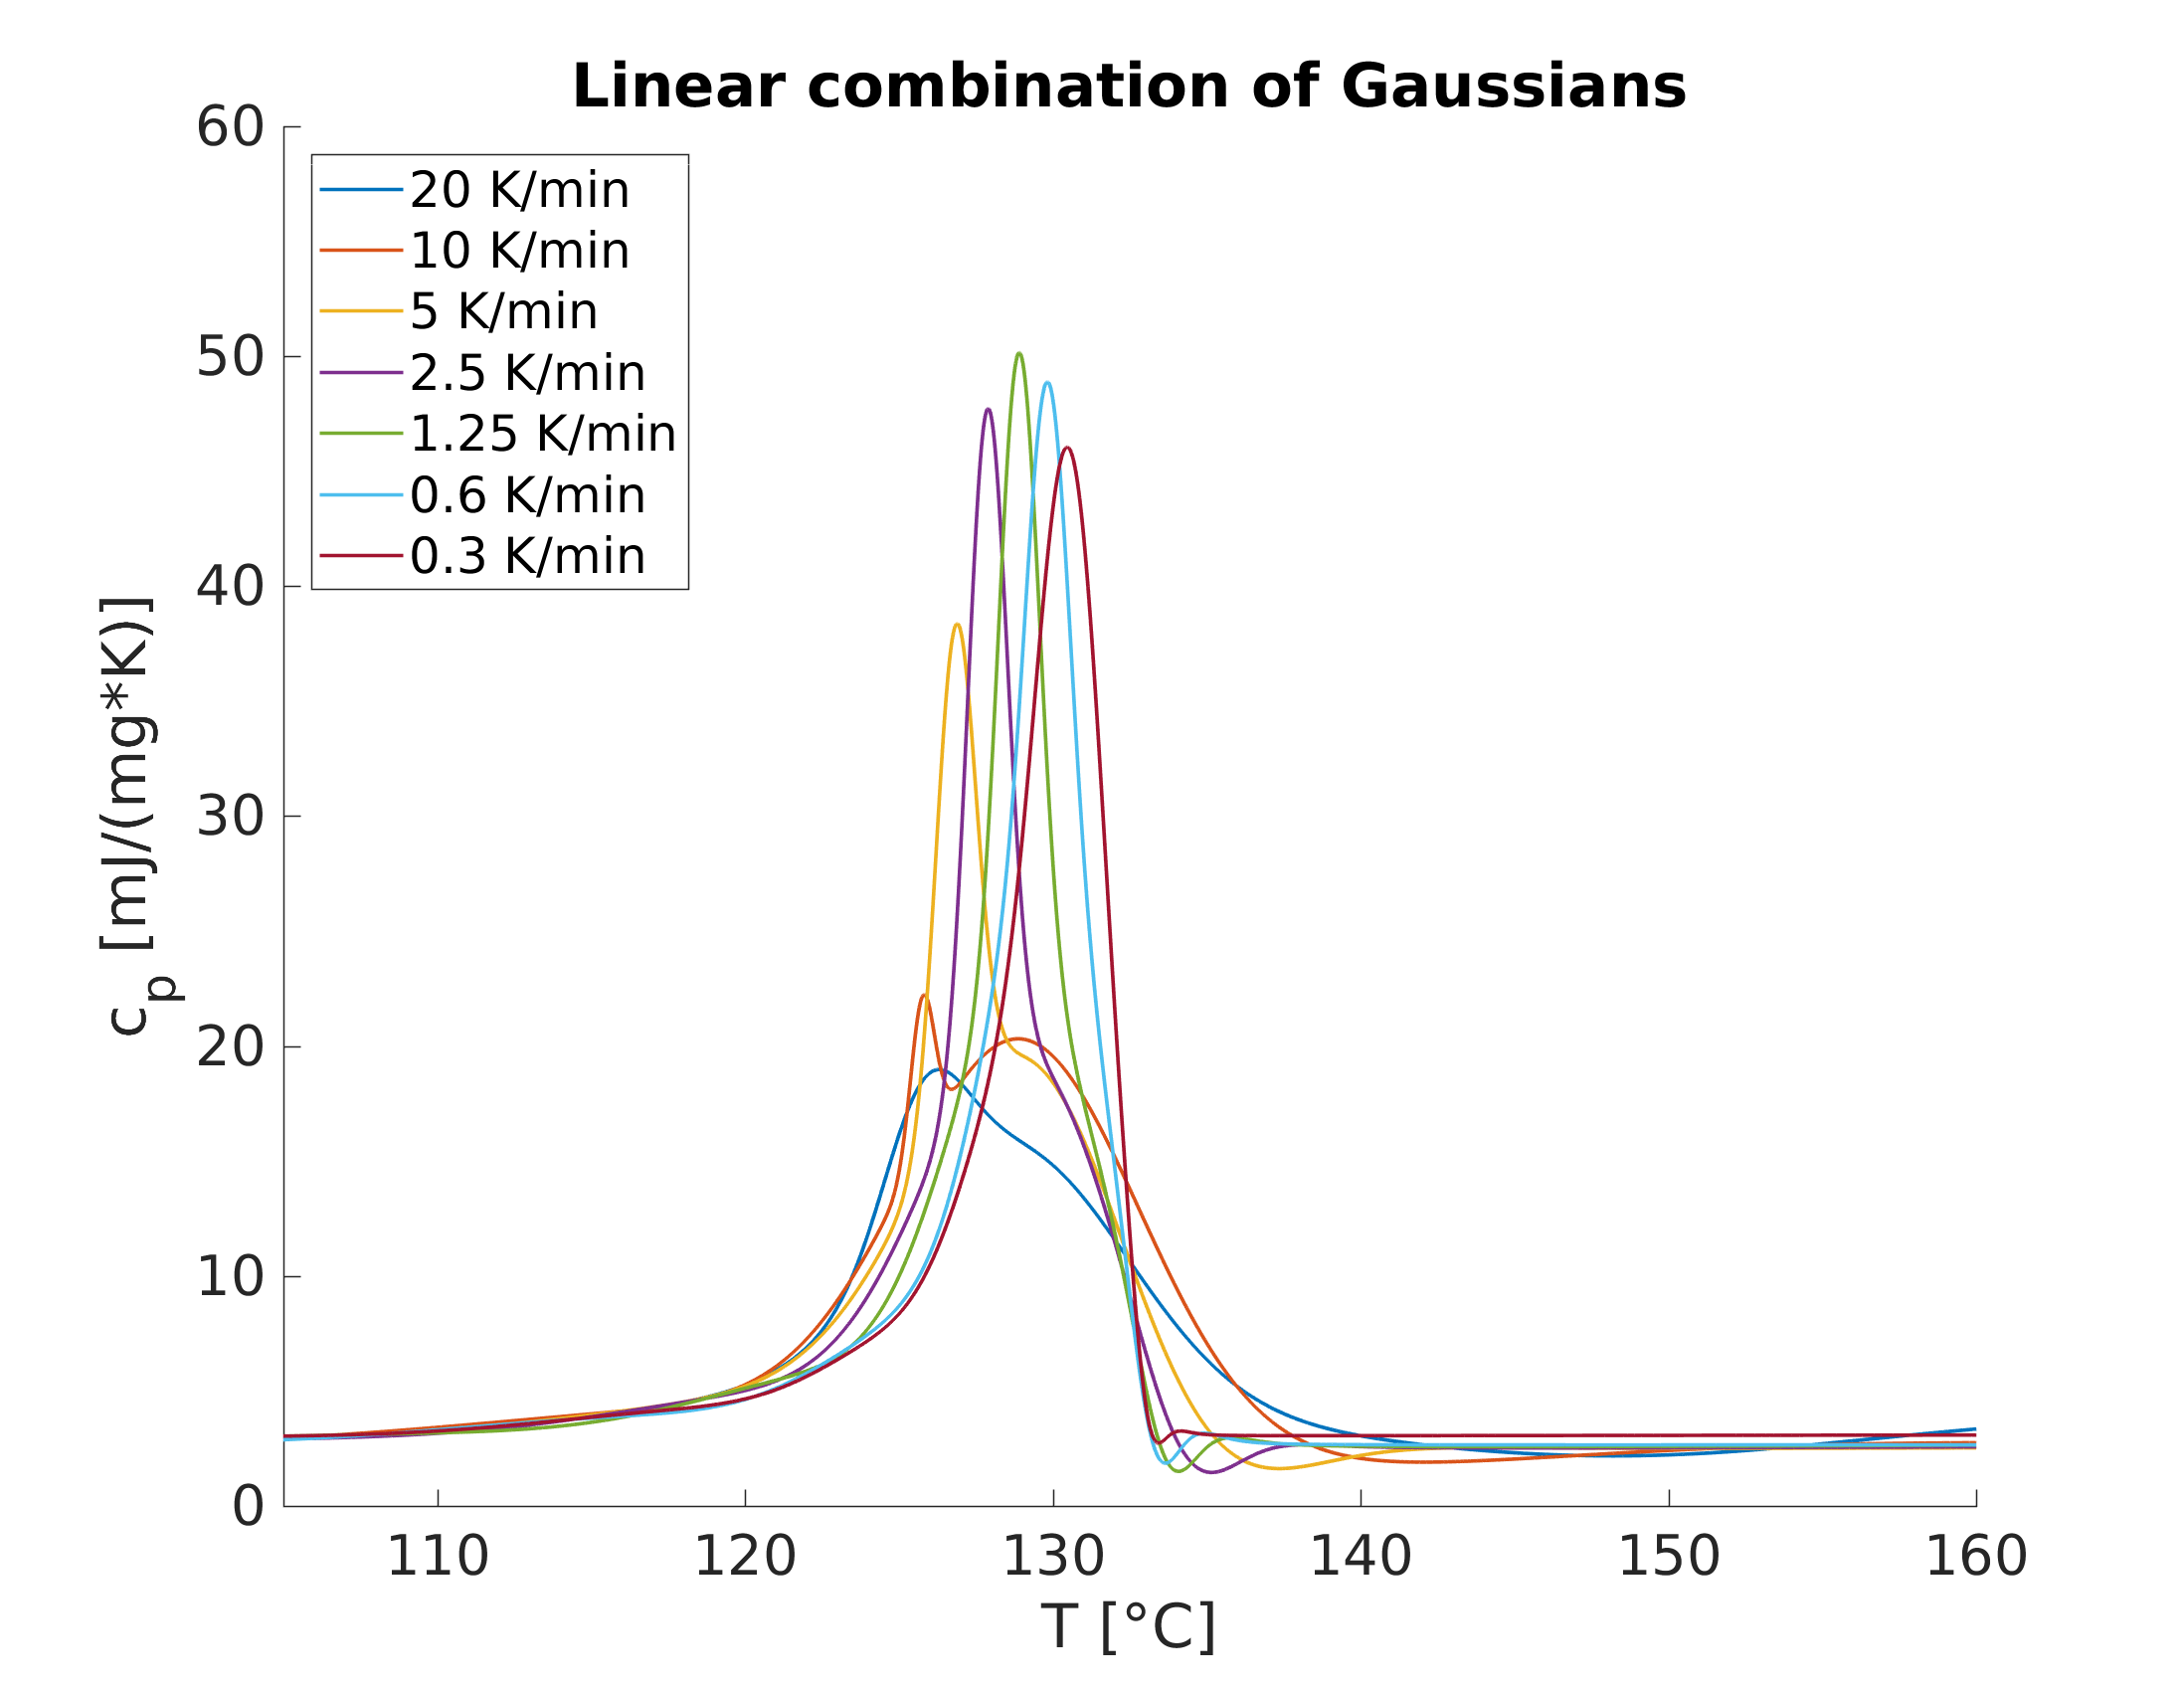
\includegraphics[width=1.\textwidth]{/home/argo/masterarbeit/vortrag/images/c_p_all_Gaussians.png}
	\end{textblock}
	
	\begin{textblock}{6.9}(8,8.7)
		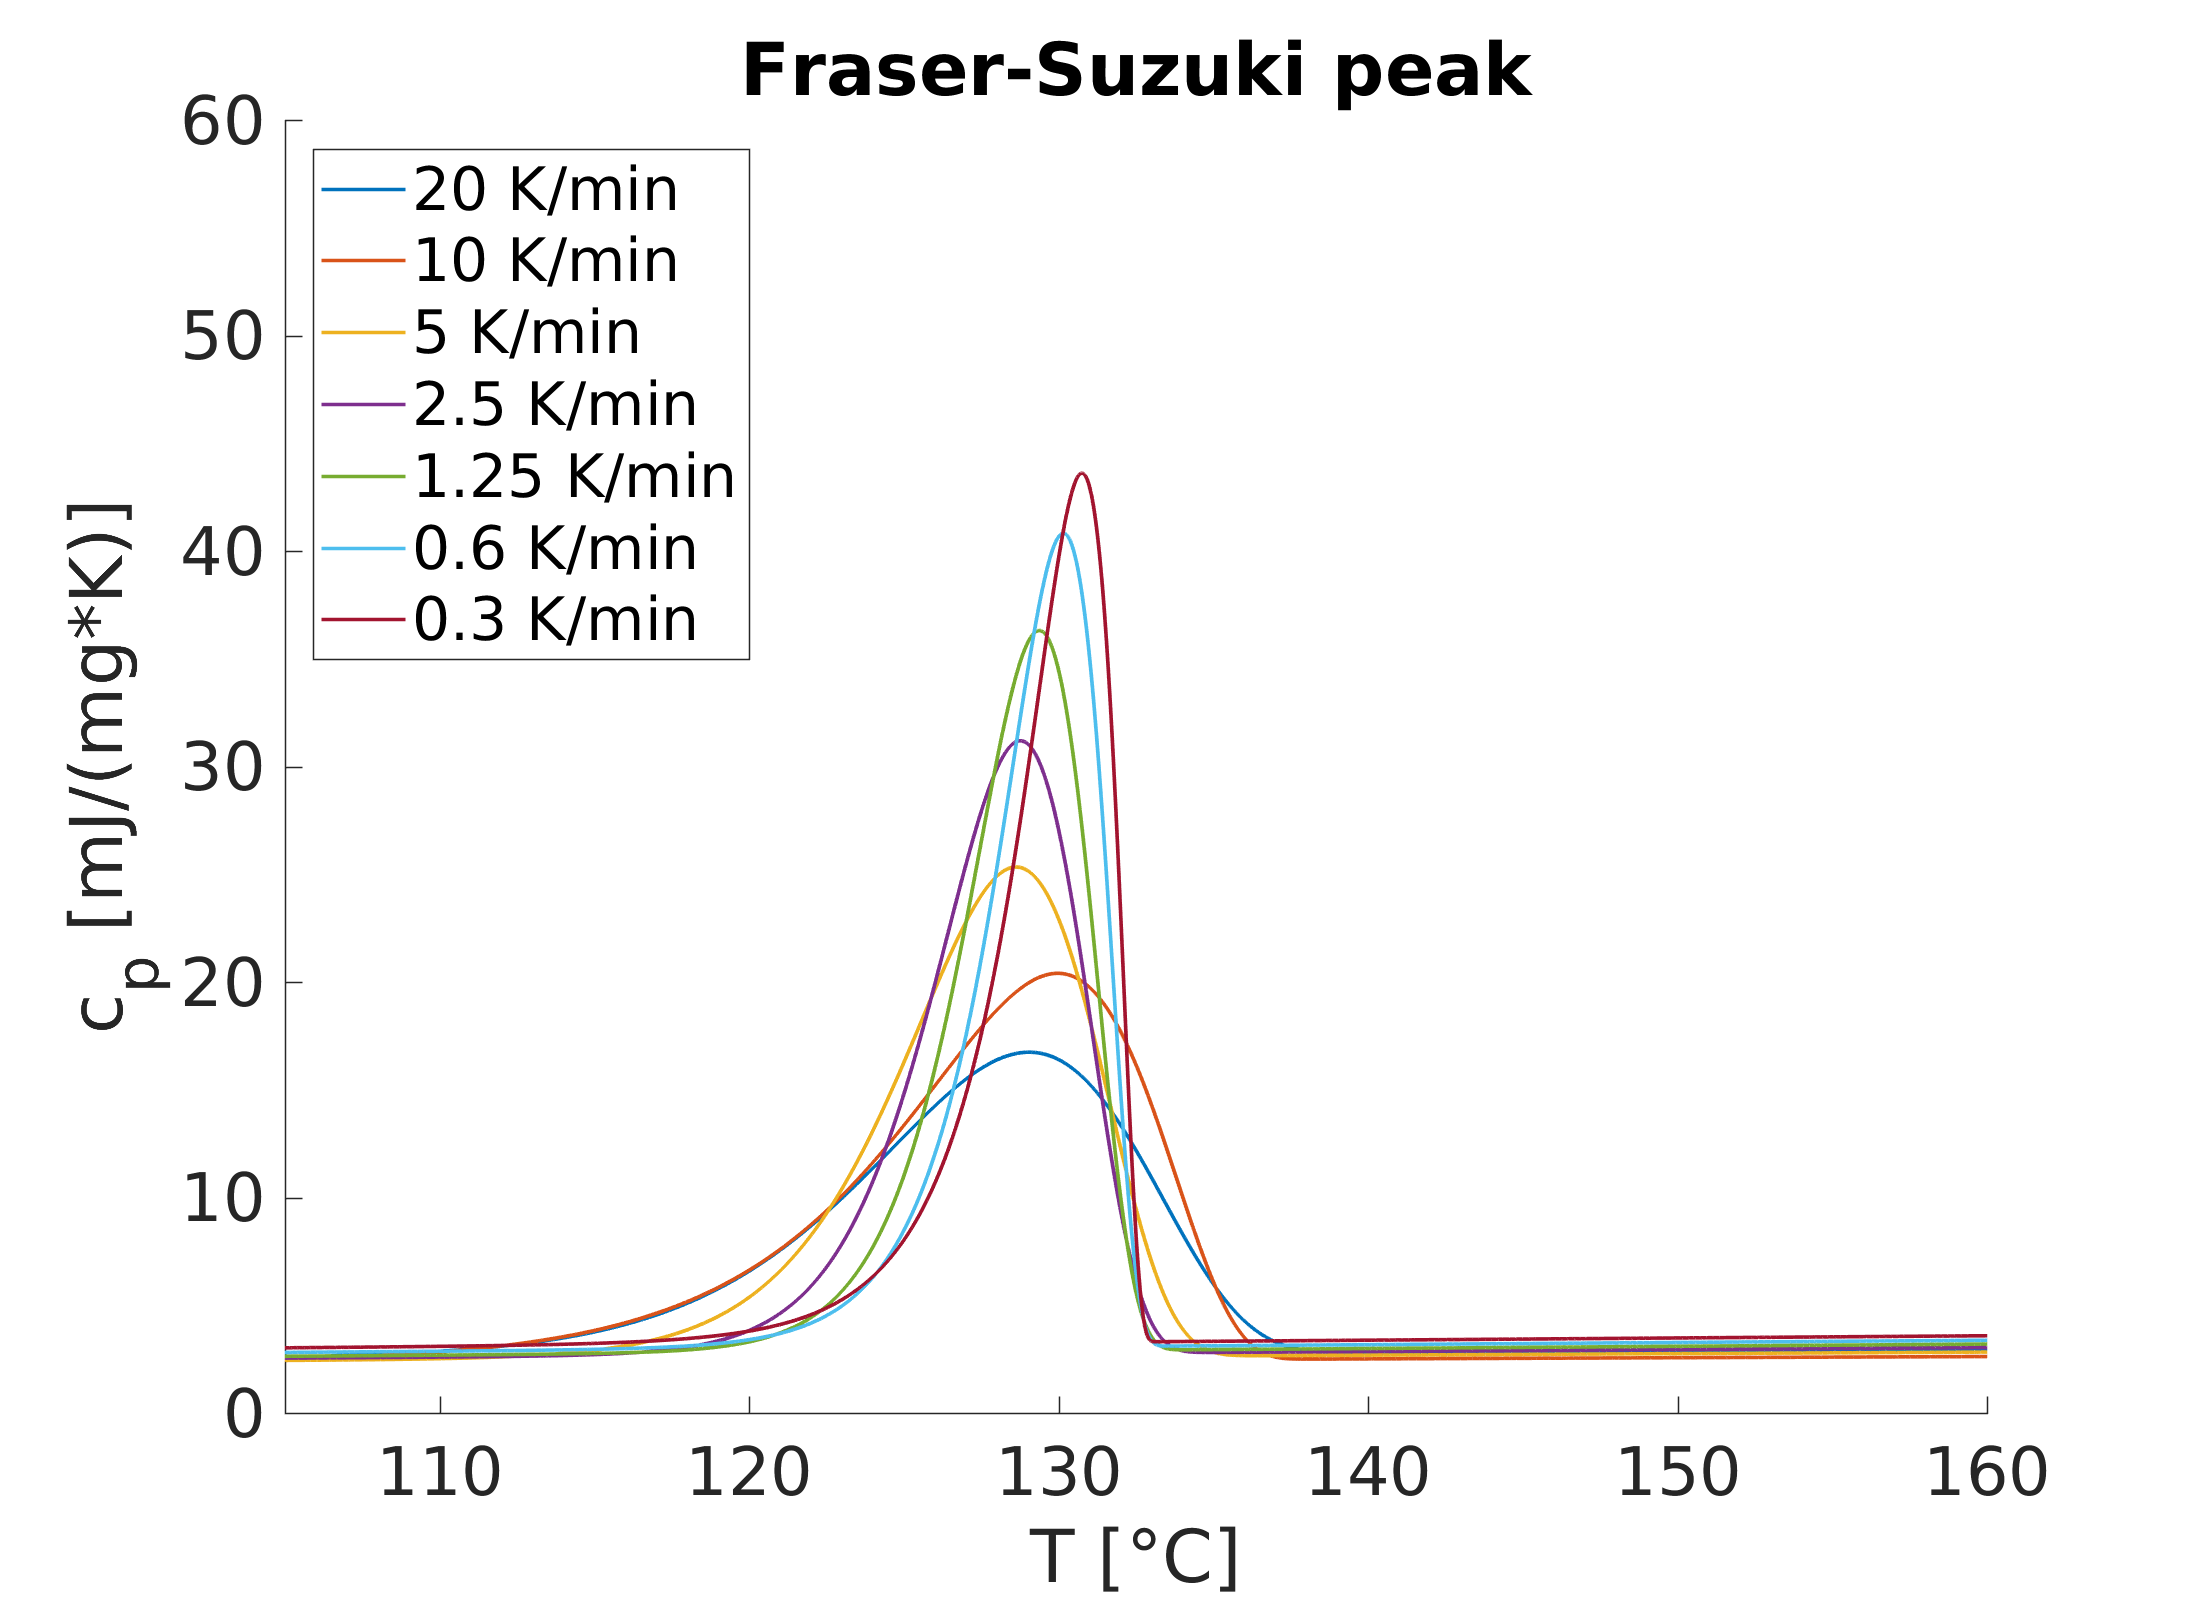
\includegraphics[width=1.\textwidth]{/home/argo/masterarbeit/vortrag/images/c_p_all_FS.png}
	\end{textblock}
	
}

%\frame{
%	\frametitle{$c_p(T)$ from parameter estimation}	
%	
%	\begin{textblock}{14}(0.,5.5)
%		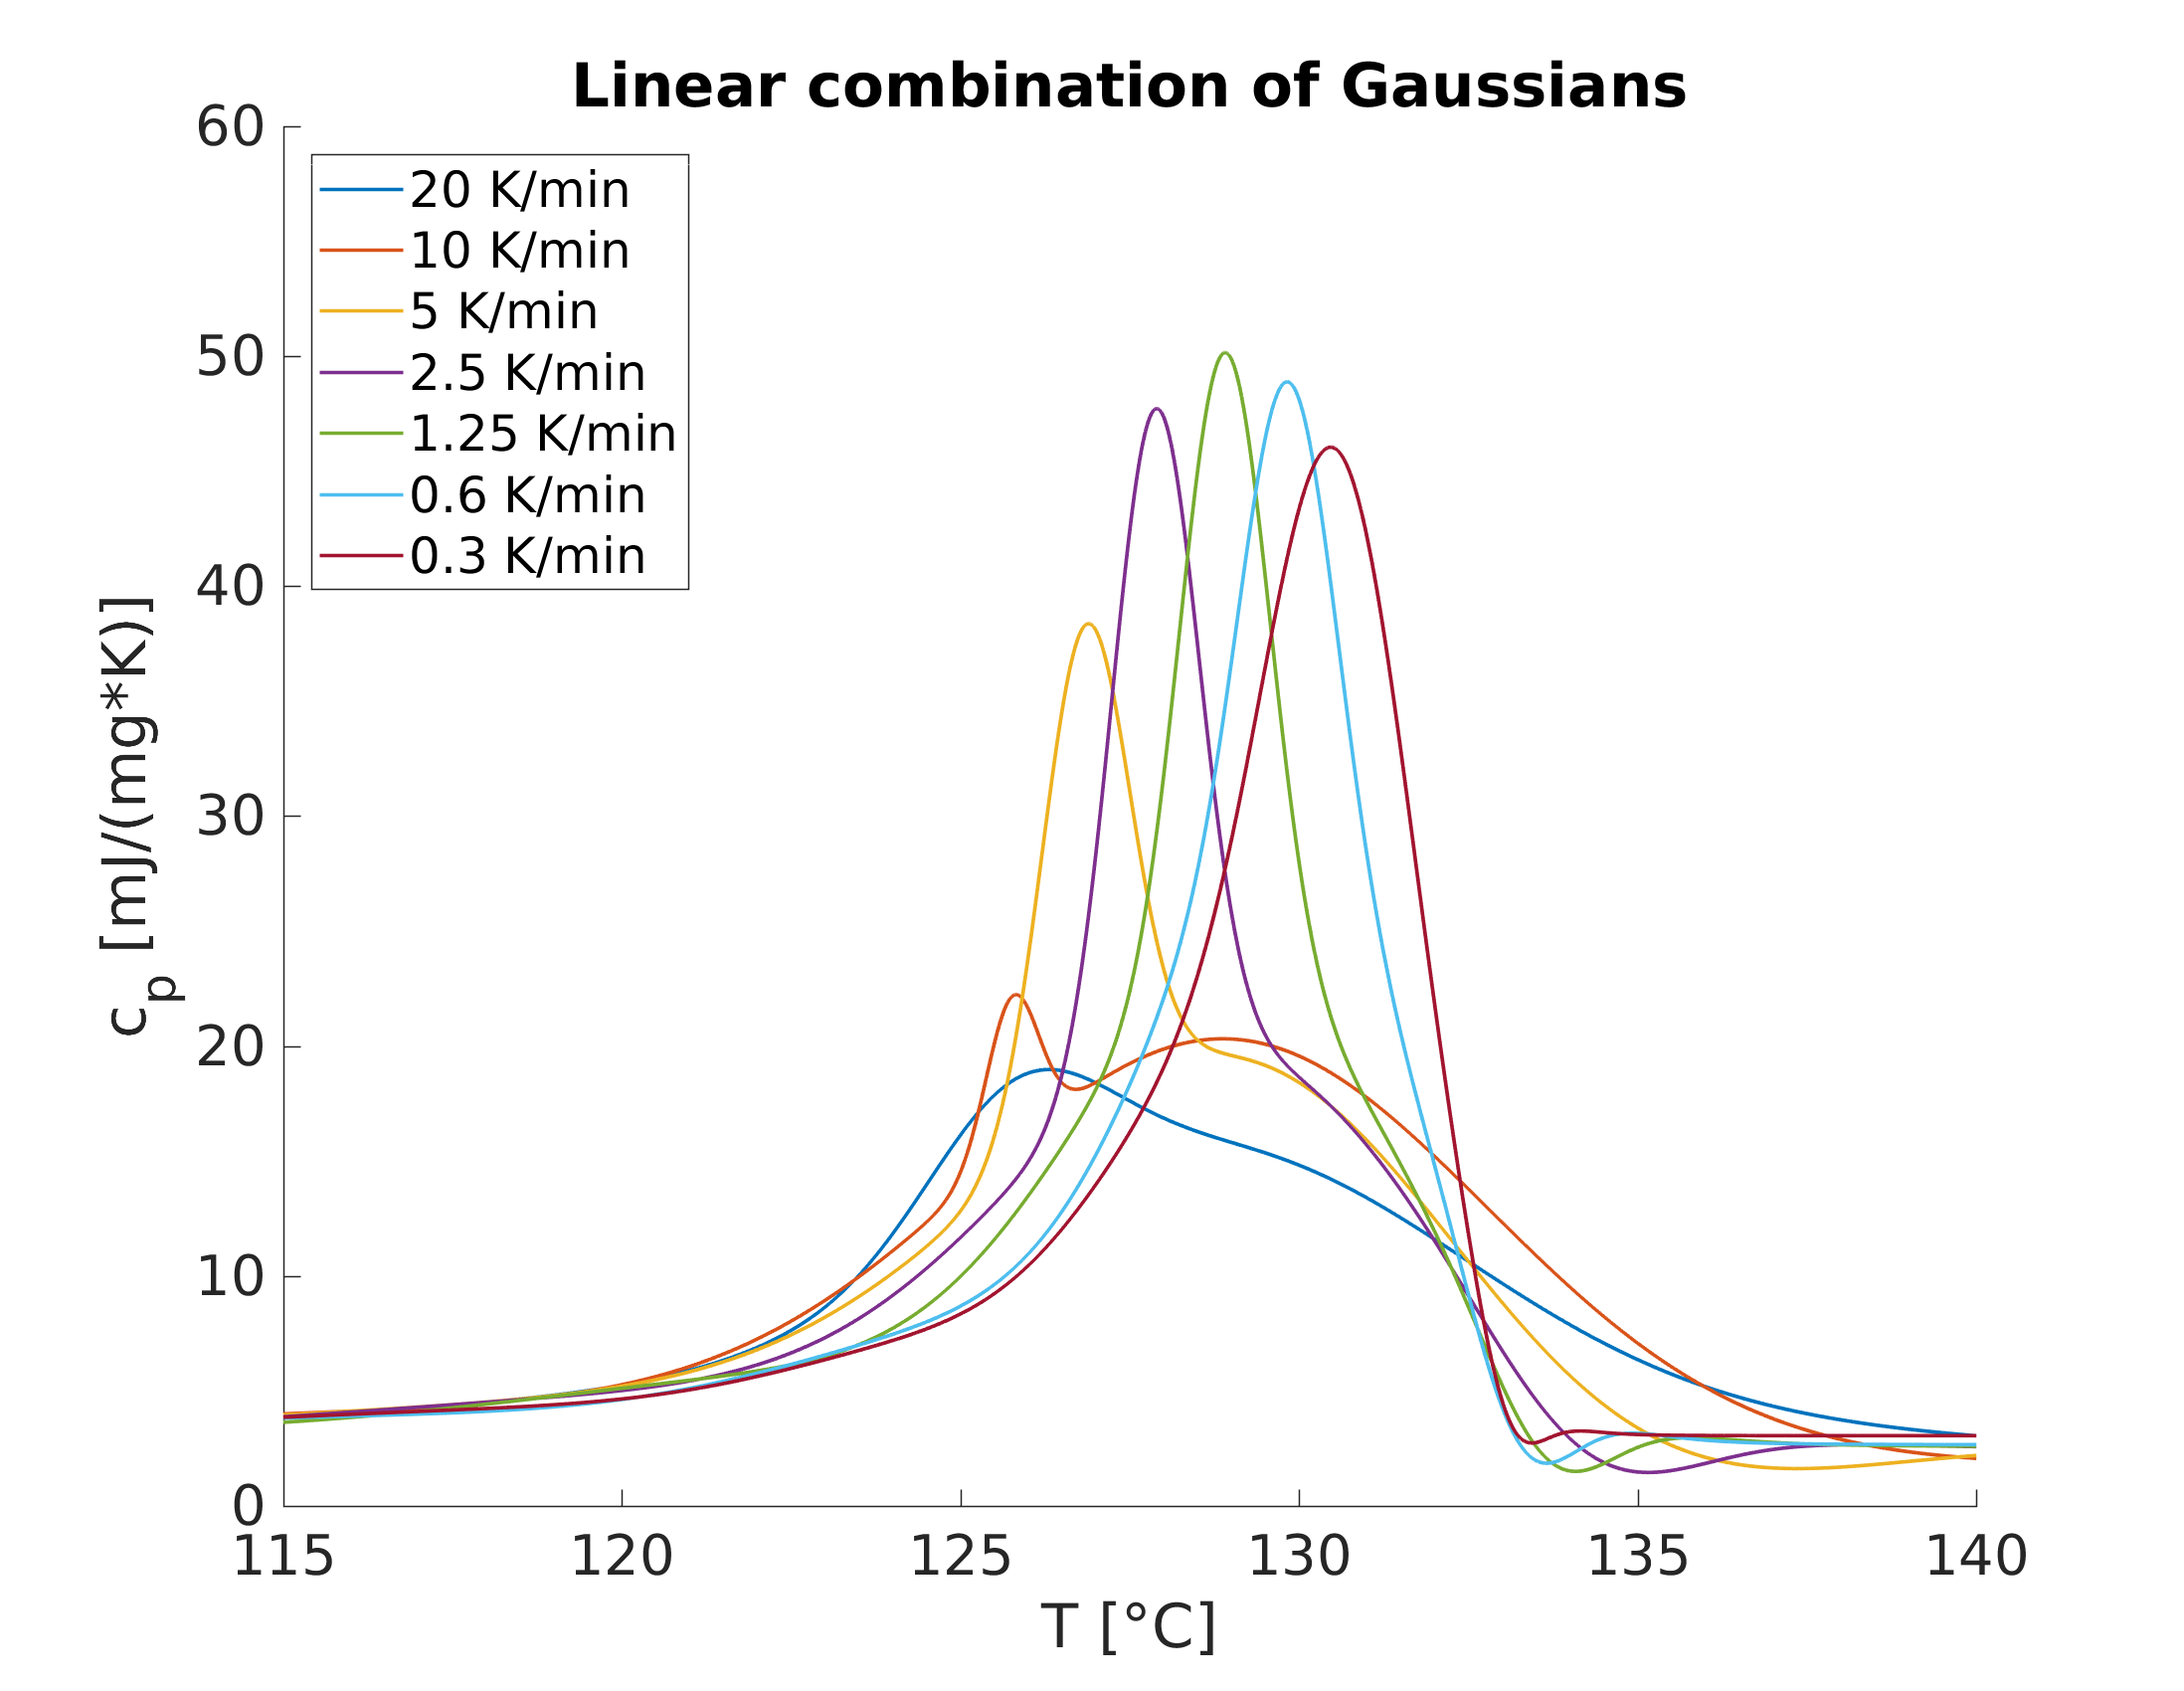
\includegraphics[width=0.6\textwidth]{/home/argo/masterarbeit/vortrag/images/c_p_all_zoom_Gaussians.png}
%	\end{textblock}
%	
%	\begin{textblock}{14}(8,5.8)
%		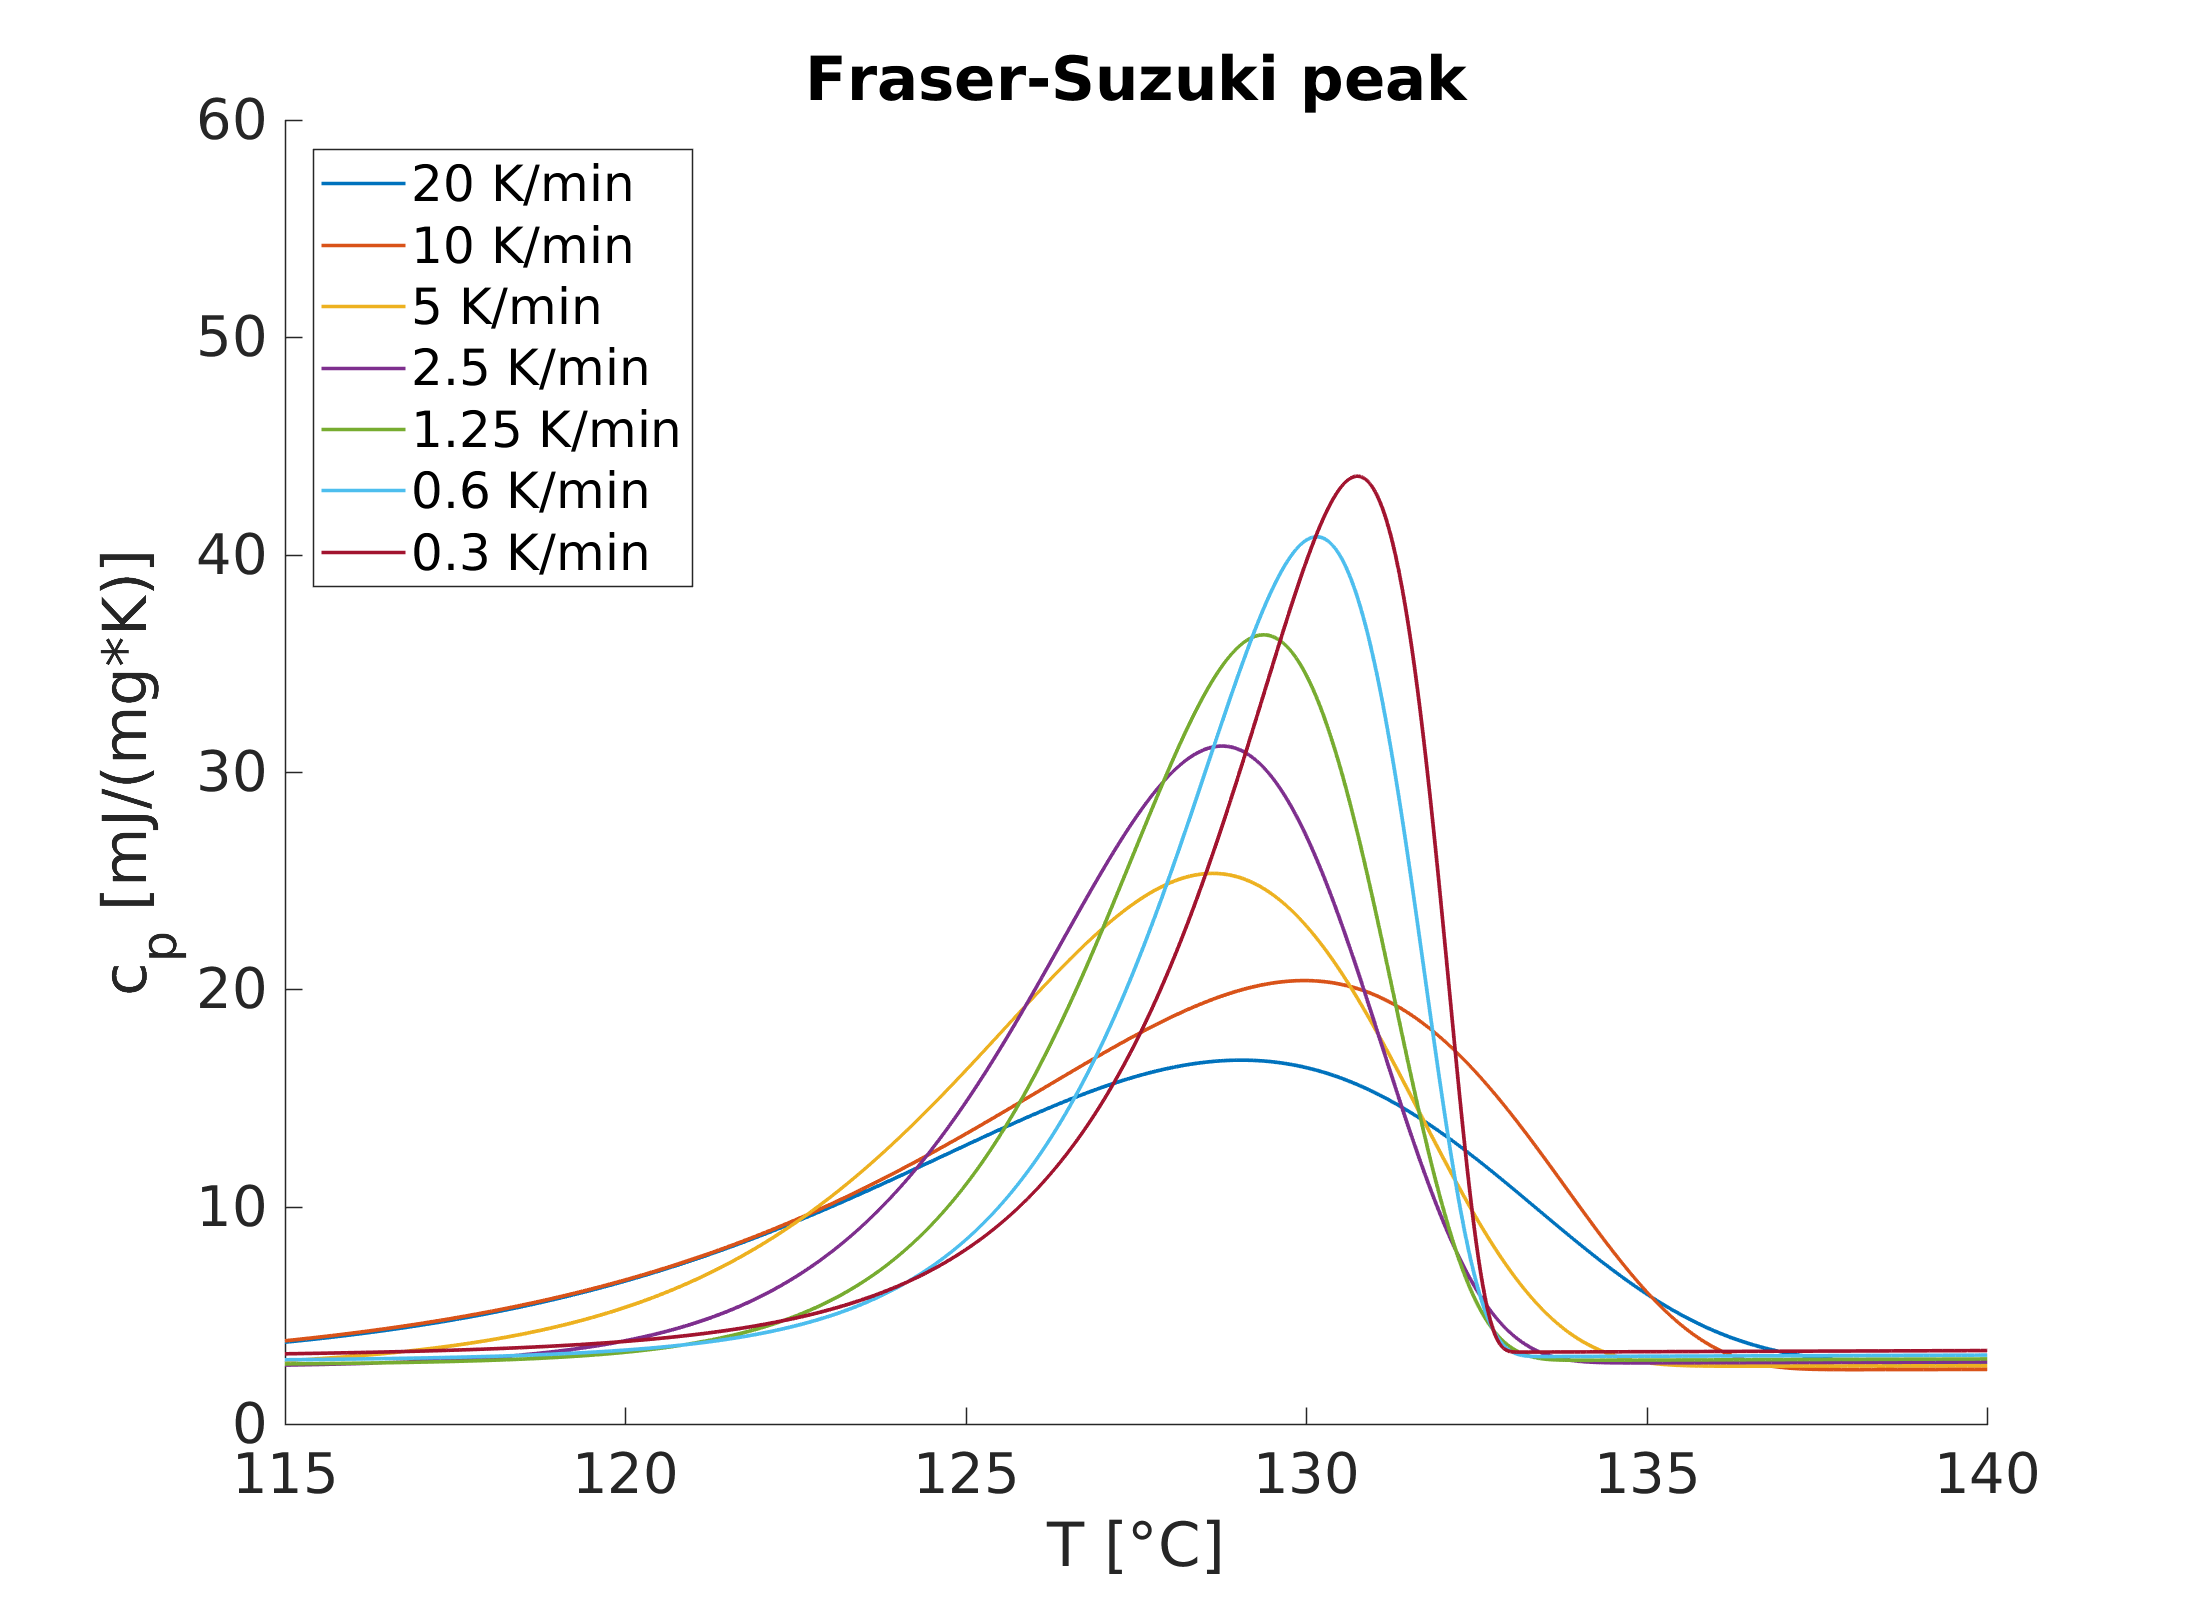
\includegraphics[width=0.6\textwidth]{/home/argo/masterarbeit/vortrag/images/c_p_all_zoom_FS.png}
%	\end{textblock}
%	
%}






\frame{
	\frametitle{Peak characteristics}
	
	\begin{textblock}{13.5}(0.,4)
		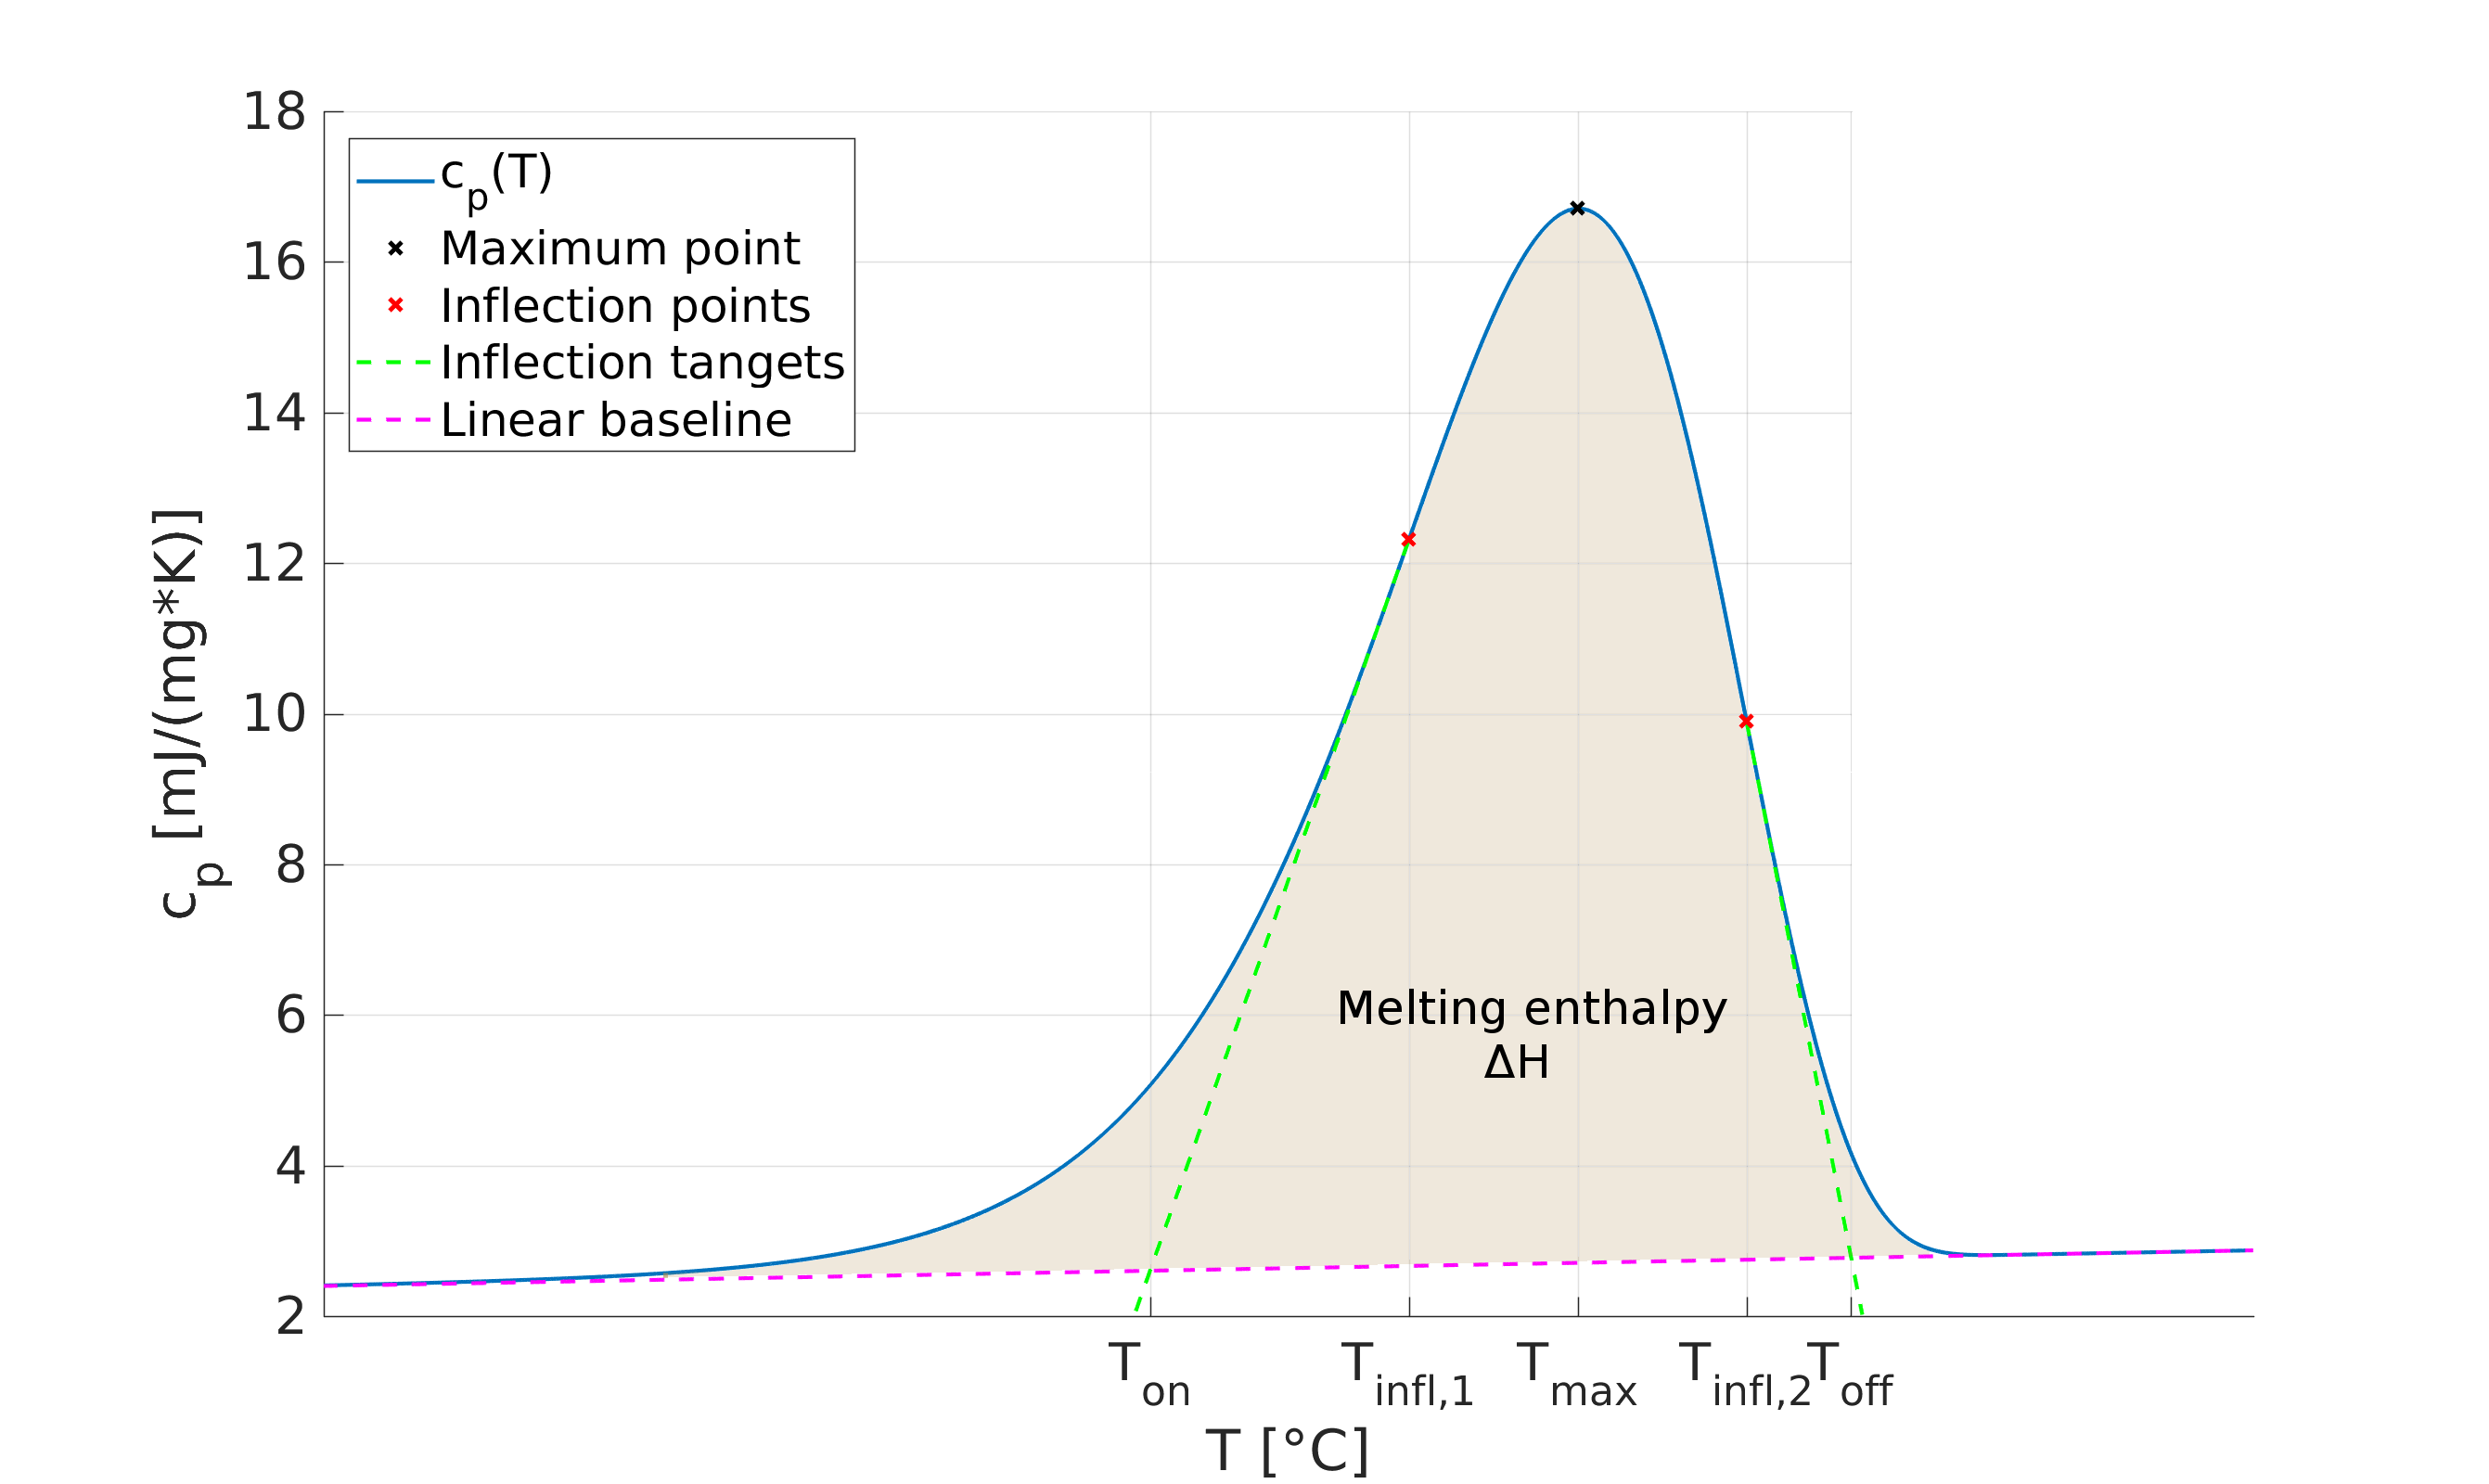
\includegraphics[width=1.\textwidth]{/home/argo/masterarbeit/vortrag/images/T_on_T_off_illustration2.png}
	\end{textblock}
	
	\begin{textblock}{6}(10,6)
		\begin{itemize}
			\item Maximum point $T_{max}$
			\item On- and offset of melting $T_{on}$, $T_{off}$
			\item Melting enthalpy $\Delta H$
		\end{itemize}
	\end{textblock}
	
}


\frame{
	\frametitle{Peak characteristics}
	
	\begin{textblock}{14}(1.,5)
		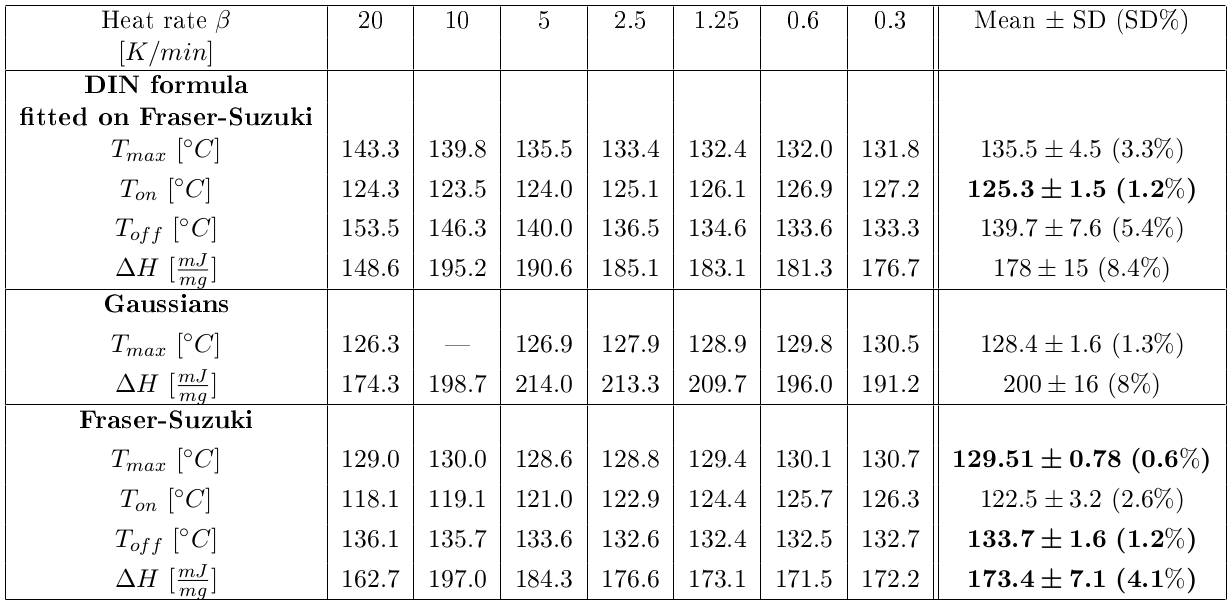
\includegraphics[width=1.\textwidth]{/home/argo/masterarbeit/vortrag/images/summary_peak_characteristics5.png}
	\end{textblock}

}






\section{Possible directions of further research}
\frame{
	\frametitle{Possible directions of further research}
	
	\begin{textblock}{14}(1,5.)
		\begin{itemize}
			\item Reason for remaining shape differences of $c_p$ from parameter estimation?
			\begin{itemize}
				\item Temperature dependent mass density $\rho_{pcm}$? \\
				$\rightarrow$ Mechanical work by volume change has to be considered
				\item Temperature dependent heat conductivity $\lambda_{pcm}$? \\
				$\rightarrow$ Nonlinear term in heat equation
				\item Model too simplified? \\
				$\rightarrow$ 2D model, crucible layer, ...
			\end{itemize}
			\item Perform parameter estimation with measurement data of another sample mass
			\item Analogous modeling of power compensated DSC
		\end{itemize}
	\end{textblock}	
}



\frame{
	\frametitle{Possible directions of further research}
	
	\begin{textblock}{14}(1,5.)
		\begin{itemize}
			\item Reason why necessary optimality condition [NOC1] could not be satisfied better, i.e. $||\nabla L||_2$ decreased further
			\item Reason for integration problems with relative local error control of forward sensitivities? \\
			$\rightarrow$ Solve variational differential equation
			\item Sensitivity generation: Why did forward mode showed to be faster than adjoint mode?
		\end{itemize}
	\end{textblock}	
}


\begin{thebibliography}{9}
\frame{
	\frametitle{References}
	
	\begin{textblock}{15}(1., 4.)
		
			\bibitem{heating_pad}
				https://de.wikipedia.org/wiki/Latentw\"{a}rmespeicher, \\
				queried 27.12.2017
			
			\bibitem{diss_dsc}
				Stefan Hiebler.
				Kalorimetrische Methoden zur Bestimmung
				der Enthalpie von Latentwärmespeichermaterialien
				während des Phasenübergangs.
				Dissertation an der technischen Universität München 
				(2006)
				
			\bibitem{nonlinear_optimiziation_wright}
				Jorge Nocedal, Stephen J. Wright.
				Numerical Optimization.
				Second Edition, 2006 Springer Science+Business Media, LLC, ISBN-13: 978-0387-30303-1
				
	\end{textblock}
	
}


\frame{
	\frametitle{References}
	

\begin{textblock}{15}(1., 4.)
	

	\bibitem{diss_bock}
		Hans Georg Bock.
		Randwertproblemmethoden zur Parameteridentifizierung in Systemen nichtlinearer Differentialgleichungen,
		Bonner Mathematische Schriften, Volume 183, Universität Bonn, 1987,
		\url{http://www.iwr.uni-heidelberg.de/groups/agbock/FILES/Bock1987.pdf}, queried 12.01.2018
	
	\bibitem{diss_jan}
		Jan Albersmeyer.
		Adjoint-based algorithms and numerical methods for sensitivity generation and optimization of large scale dynamic systems.
		\url{http://www.ub.uni-heidelberg.de/archiv/11651}.
		(2010)
	
\end{textblock}
	
	
}

\end{thebibliography}	
	


\frame{
	\frametitle{Summary of thesis contents}
	
	\begin{textblock}{15}(0.5,4.)
	\begin{itemize}
		\item Development and implementation of heat flux DSC -- 1D model capable of reproducing heat fluxes similar to those measured
		\item Spatial grid construction with error analysis
		\item Sensitivity generation by both finite differences and IND + AD
		\item Parameter estimation with three different parametrizations (NURBS, Gaussians, Fraser-Suzuki) including statistical a posteriori analysis and peak characteristics analysis \\
		$\rightarrow$ Distinct reduction of smearing in specific heat capacity
		\item Gauss-Newton method implemented with linesearch and active set strategy for parameter bounds \\
		$\rightarrow$ Examination of optimization process
		\item Analytical solution of heat flux DSC reference side
	\end{itemize}
	\end{textblock}
		
	
	
	
}



\frame{
	
\begin{textblock}{15}(0.5,2.5)
	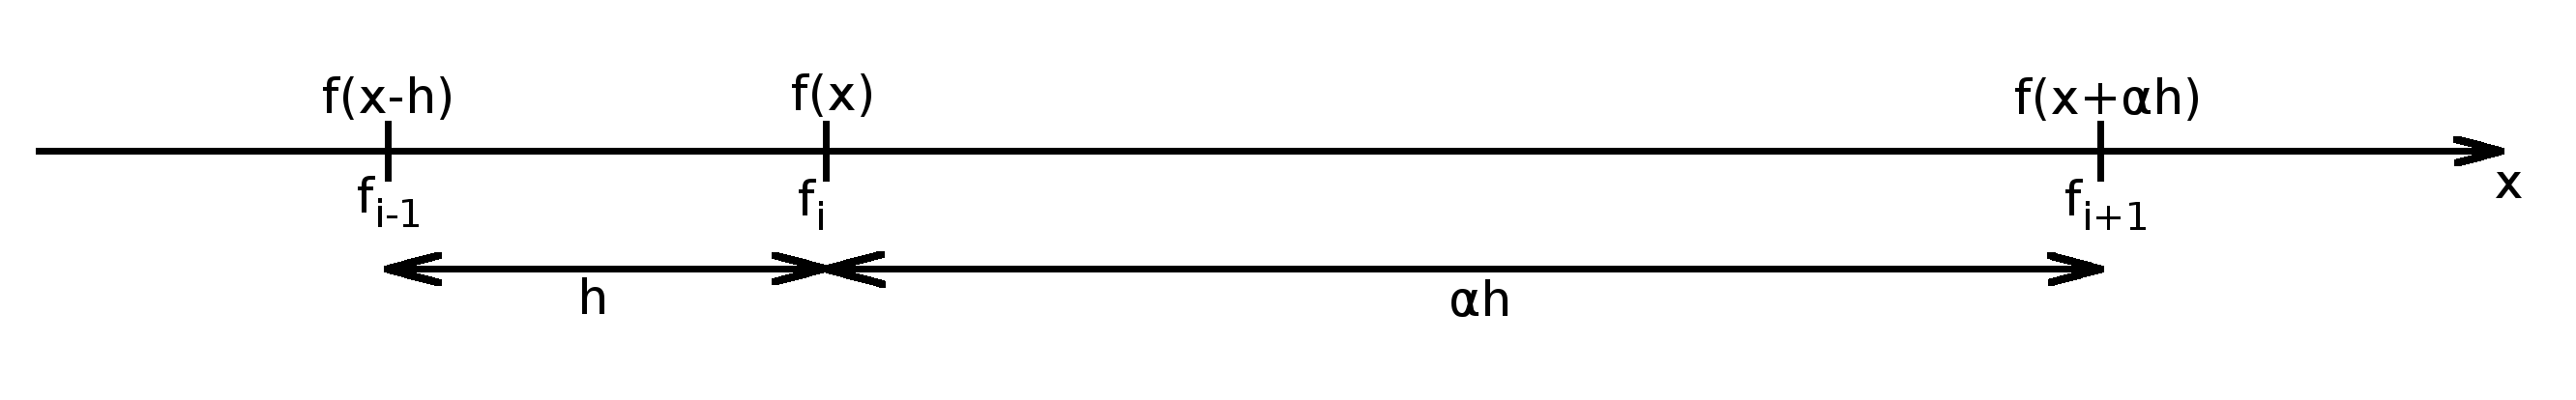
\includegraphics[width=1.0\textwidth]{/home/argo/masterarbeit/thesis/images/2nd_derivative_2-point_formula_illustration.png}
\end{textblock}
	
\begin{textblock}{15}(0.2,6)

	\begin{align}
		f(x-h) = & f(x) - h \cdot \frac{\partial f}{\partial x}(x) + \frac{h^2}{2} \cdot \frac{\partial^2 f}{\partial^2 x}(x) + \mathcal{O}(h^3) \label{eq:finite_differences_taylor_exp_non-homogenous_1} \\
		f(x+\alpha h) = & f(x) + \alpha h \cdot \frac{\partial f}{\partial x}(x) + \frac{\alpha^2 h^2}{2} \cdot \frac{\partial^2 f}{\partial^2 x}(x) + \mathcal{O}(h^3) \\[3ex]
		\Leftrightarrow \frac{\partial^2 f}{\partial^2 x}(x) = & \frac{1}{h^2} \left[ \frac{2}{1+\alpha} f(x-h) - \frac{2}{\alpha} f(x) + \frac{2}{\alpha (\alpha+1)} f(x+\alpha h) \right] + \mathcal{O}(h) 
	\end{align}

\end{textblock}

}
	
\end{document}